\documentclass[12pt]{article}
\usepackage{amsmath}
\usepackage{amsthm}
\usepackage{amssymb}
\usepackage{euscript}
\usepackage{mathrsfs}
\usepackage{bm}
\usepackage{enumitem}
\usepackage{tikz}
\usepackage{mathtools}
\usepackage{float}
\usepackage{hyperref}
\usepackage{boldline}
\usepackage{indentfirst}
\usepackage{environ}
\usepackage{courier}
\usetikzlibrary{positioning}

\renewcommand{\labelitemii}{$\vartriangleright$}
\renewcommand{\labelitemiv}{$\Join$}

\makeatletter
\newsavebox{\measure@tikzpicture}
\NewEnviron{scaletikzpicturetowidth}[1]{%
  \def\tikz@width{#1}%
  \def\tikzscale{1}\begin{lrbox}{\measure@tikzpicture}%
  \BODY
  \end{lrbox}%
  \pgfmathparse{#1/\wd\measure@tikzpicture}%
  \edef\tikzscale{\pgfmathresult}%
  \BODY
}
\makeatother

\numberwithin{equation}{section}

\hypersetup{
    colorlinks=true,
    % linkcolor=blue,
    linkcolor=[RGB]{0,0,128},
    % filecolor=[RGB]{0,0,128},
    filecolor=magenta,
    urlcolor=cyan,
    citecolor = [RGB]{128,0,128}
}

\newcommand{\myref}[2]{\hyperref[#2]{#1 \ref*{#2}}}
\newcommand{\myrefT}[1]{\hyperref[#1]{Theorem \ref*{#1}}}
\newcommand{\myrefP}[1]{\hyperref[#1]{Proposition \ref*{#1}}}
\newcommand{\myrefL}[1]{\hyperref[#1]{Lemma \ref*{#1}}}
\newcommand{\myrefD}[1]{\hyperref[#1]{Definition \ref*{#1}}}
\newcommand{\myrefn}[3]{\hyperref[#2]{#1 \ref*{#2} (#3)}}

% \input{dynkinMacros.tex}
% \input{dynkinEMacros.tex}
% \renewcommand{\qedsymbol}{}
\newcommand{\ssm}{\smallsetminus}

\newcommand{\para}[1]{\noindent\underline{#1}.}

\newcommand{\ti}{$\tau\textnormal{-invariant}$}
\newcommand{\prim}{\textnormal{Prim}_{\lambda}(\textnormal{U}(\gf))}

\newcommand{\ve}{\varepsilon}
\newcommand{\veo}{\varepsilon_1}
\newcommand{\vet}{\varepsilon_2}
\newcommand{\vei}{\varepsilon_i}
\newcommand{\vp}{\varphi}

% \newcommand{\inr}{\textnormal{In}^R}
% \newcommand{\inl}{\textnormal{In}^L}
% \newcommand{\inc}{\textnormal{In}}
% \renewcommand{\sc}{\textnormal{SC}}
% \newcommand{\re}{\textnormal{Re}}

\newcommand{\ag}{\alpha}
\newcommand{\bg}{\beta}
\newcommand{\g}{\gamma}
\newcommand{\dg}{\delta}
\newcommand{\rg}{\rho}
\newcommand{\kg}{\kappa}
\newcommand{\sg}{\sigma}
\newcommand{\tg}{\tau}
\renewcommand{\lg}{\lambda}

\renewcommand{\gg}{$\gamma \ $}
\newcommand{\ga}{$\alpha \ $}
\newcommand{\gt}{$\tau $}
\renewcommand{\(}{(\gamma)}
\newcommand{\atg}{\tilde\alpha}
\newcommand{\ags}[1]{{\ag_{#1}}}
\newcommand{\ao}{{\ag_1'}}

\newcommand{\gf}{\mathfrak g}
\newcommand{\hf}{\mathfrak h}

% needs a new name
%\newcommand{\th}[1]{{$\text{\it #1 }^{\underline{\textnormal{th}}}$}}
\renewcommand{\sf}{\mathscr F}
\newcommand{\dsf}{$\sf$}
\newcommand{\st}{\mathscr T}
% needs a new name  -- ok?
\newcommand{\so}[1]{\mathscr #1}


\newcommand{\snn}{{\mathscr S(n,n)}}
\newcommand{\smm}{{\mathscr S(M^L,M^R)}}
\renewcommand{\tan}{\mathscr T_A(n)}
\newcommand{\tn}{\mathscr T(n)}
\newcommand{\dtn}{$\tn$}
\newcommand{\tm}{\mathscr T(M)}
\newcommand{\dtm}{$\tm$}
\newcommand{\tcsn}{\mathscr T_C^S(n)}
\newcommand{\tbsn}{\mathscr T_B^S(n)}
\newcommand{\tsn}[1]{\mathscr T_#1(n)}
\newcommand{\tsm}[1]{\mathscr T_#1(M)}
\newcommand{\tnn}{\mathscr T(n,n)}
\newcommand{\tmm}{\mathscr T(M^L,M^R)}
\newcommand{\tkmm}{\mathscr T_K(M^L,M^R)}
\newcommand{\tsnn}[1]{\mathscr T_#1(n,n)}
\newcommand{\tsmm}[1]{\mathscr T_#1(M^L,M^R)}
\newcommand{\tdnn}{\mathscr T_D(n,n)}
\newcommand{\tdmm}{\mathscr T_D(M^L,M^R)}
\newcommand{\tdn}{\mathscr T_D(n)}
\newcommand{\tdm}{\mathscr T_D(M)}
\newcommand{\tcnn}{\mathscr T_C(n,n)}
\newcommand{\tcmm}{\mathscr T_C(M^L,M^R)}
\newcommand{\tcn}{\mathscr T_C(n)}
\newcommand{\tcm}{\mathscr T_C(M)}
\newcommand{\cm}{\mathscr C(M)}
\newcommand{\dm}{\mathscr D(M)}

\newcommand{\snnp}{\mathscr S'(n,n)}
\newcommand{\smmp}{\mathscr S'(M^L,M^R)}
\newcommand{\snnpp}{\mathscr S''(n,n)}
\newcommand{\smmpp}{\mathscr S''(M^L,M^R)}
\newcommand{\tnnp}{\mathscr T'(n,n)}
\newcommand{\tmmp}{\mathscr T'(M^L,M^R)}
\newcommand{\tnnpp}{\mathscr T''(n,n)}
\newcommand{\tmmpp}{\mathscr T''(M^L,M^R)}
\newcommand{\tdnnp}{\mathscr T_D'(n,n)}
\newcommand{\tdmmp}{\mathscr T_D'(M^L,M^R)}
\newcommand{\tdnnpp}{\mathscr T_D''(n,n)}
\newcommand{\tdmmpp}{\mathscr T_D''(M^L,M^R)}


\newcommand{\talb}{T_{\alpha \beta}}
\newcommand{\tai}{T_{\alpha_i,\alpha_{i+1}}}
\newcommand{\tap}{T_{\alpha_{i+1},\alpha_i}}
\newcommand{\tao}{T_{\alpha_1,\alpha_2}}
\newcommand{\tat}{T_{\alpha_2,\alpha_1}}

% new
\newcommand{\talbLeft}{T^L_{\alpha \beta}}
\newcommand{\talbRight}{T^R_{\alpha \beta}}

\newcommand{\ot}{\overline T}
\newcommand{\og}{\overline{\gamma}}

\newcommand{\sij}{{S_{ij}}}
\renewcommand{\ss}[2]{{S_{#1,#2}}}
% \def\ss#1#2{S_{#1,#2}}

\newcommand{\im}{{i-1}}
% \renewcommand{\ip}{{i+1}}
\newcommand{\ip}{{i+1}}
\newcommand{\imm}{{i-2}}
\newcommand{\ipp}{{i+2}}
\newcommand{\jm}{{j-1}}
\newcommand{\jp}{{j+1}}
\newcommand{\jmm}{{j-2}}
\newcommand{\jpp}{{j+2}}

\renewcommand{\tt}{\tau (T)}
\newcommand{\abe}{{$\{\ag,\bg\}=\{\ag_i,\ag_\ip\}$}}

\newcommand{\bt}{\mathbf T}
\newcommand{\bto}{\mathbf T_1}
\newcommand{\btt}{\mathbf T_2}
\newcommand{\obt}{\overline\bt}
\newcommand{\obto}{\overline\bt_1}
\newcommand{\obtt}{\overline\bt_2}
\newcommand{\tbt}{\tilde\bt}
\newcommand{\tbto}{\tilde\bto}
\newcommand{\tbtt}{\tilde\btt}
\newcommand{\pbt}{(\bto,\btt)}
\newcommand{\pbtp}{(\bto',\btt')}
\newcommand{\pobt}{(\obto,\obtt)}
\newcommand{\pbts}[1]{(\bto^{#1},\btt^{#1})}
\newcommand{\pobts}[1]{(\obto^{#1},\obtt^{#1})}
\newcommand{\pobtp}{(\obto',\obtt')}

\newcommand{\lo}{(\bto,\bt)}
\newcommand{\lop}{(\bto',\bt)}
\newcommand{\ls}[1]{(\bt_#1,\bt)}
\newcommand{\lsp}[1]{(\bt_#1',\bt)}
\newcommand{\ol}{(\obt_1,\obt)}

\newcommand{\be}{\mathbf E}
\newcommand{\bs}{\mathbf S}
\newcommand{\bl}{\mathbf L}
\newcommand{\br}{\mathbf R}
% \renewcommand{\op}{\bar P}
\newcommand{\op}{\bar P}
\newcommand{\pe}{P_e}

\newcommand{\oc}{\overline c}
\newcommand{\cL}{\prescript{L}{}{c}}
\newcommand{\cR}{\prescript{R}{}{c}}
\newcommand{\bc}{\mathbf c}
\newcommand{\bcL}{\prescript{L}{}{\bc}}
\newcommand{\bcR}{\prescript{R}{}{\bc}}
\newcommand{\overbc}{\overline{\mathbf c}}
\newcommand{\overcL}{\prescript{L}{}{\overline c}}
\newcommand{\overcR}{\prescript{R}{}{\overline c}}
\newcommand{\overbcL}{\prescript{L}{}{\overbc}}
\newcommand{\overbcR}{\prescript{R}{}{\overbc}}

% \newcommand{\sha}{{\textnormal{Shape}}}
\newcommand{\cs}{{c.s.p.b.}}
% \newcommand{\OC}{{\textnormal{OC}}}
% \newcommand{\OCS}{{\textnormal{OC*}}}
\newcommand{\Sf}{S_f}
\newcommand{\Sb}{S_b}
\newcommand{\nh}{n_h}
\newcommand{\nv}{n_v}
\newcommand{\rinf}{\rg_{\inf}}
\newcommand{\rsup}{\rg_{\sup}}

\newcommand{\ec}{\underset {ec}\sim}
\newcommand{\gtl}{\underset {GTL}\sim}
\newcommand{\en}{\underset {n}\sim}
\newcommand{\enm}{\underset {n-1}\sim}
\newcommand{\eqm}{\underset {m}\sim}
\newcommand{\eqmm}{\underset {m-1}\sim}
\newcommand{\ez}{\underset {0}\sim}
\newcommand{\gtr}{\underset {GTR}\sim}
\renewcommand{\gt}{\underset {GT}\sim}
\newcommand{\ngtl}{\underset {GTL}\nsim}
\newcommand{\jl}{\underset {JL}\sim}
\newcommand{\jr}{\underset {JR}\sim}
\newcommand{\kll}{\underset {KLL}\sim}
\newcommand{\klr}{\underset {KLR}\sim}

\newcommand{\fo}{F_1}
\newcommand{\ft}{F_2}
\newcommand{\fot}{\tilde\fo}
\newcommand{\ftt}{\tilde\ft}

\newcommand{\bi}{{\it b}){\it i})}
\newcommand{\bii}{{\it b}){\it ii})}

\newcommand{\sig}{\Sigma}
\newcommand{\tsl}{T_\Sigma^L}
\newcommand{\tspl}{T_{\Sigma'}^L}
\newcommand{\tssl}[1]{T_{\Sigma^#1}^L}
\newcommand{\tssbl}[1]{T_{\Sigma_#1}^L}
\newcommand{\ts}{T_\Sigma}
\newcommand{\tsp}{T_{\Sigma'}}
\newcommand{\tss}[1]{T_{\Sigma^#1}}
\newcommand{\tssb}[1]{T_{\Sigma_#1}}
\newcommand{\pin}{$\Pi\ssm\{\ag_n\}$}
\newcommand{\pc}{\phi_C}
% \newcommand{\pd}{{\phi_D}}
\newcommand{\il}{I_\lg}

\newcommand{\te}[1]{\textnormal{#1}}

\newcommand{\plainTL}{\prescript{L}{}{T}}
\newcommand{\plainTR}{\prescript{R}{}{T}}

\newcommand{\tL}{\prescript{L}{}{\bt}}
\newcommand{\tR}{\prescript{R}{}{\bt}}
\newcommand{\pairTLR}{(\tL,\tR)}
\newcommand{\pairTLRPrime}{(\tL',\tR')}
\newcommand{\pairTLRSub}[1]{(\tL_{#1},\tR_{#1})}
\newcommand{\pairTLRPrimeSub}[1]{(\tL'_{#1},\tR'_{#1})}

\newcommand{\overTL}{\prescript{L}{}{\obt}}
\newcommand{\overTR}{\prescript{R}{}{\obt}}
\newcommand{\overPairTLR}{(\overTL,\overTR)}
\newcommand{\overPairTLRPrime}{(\overTL',\overTR')}
\newcommand{\overPairTLRSub}[1]{(\overTL_{#1},\overTR_{#1})}
\newcommand{\overPairTLRPrimeSub}[1]{(\overTL'_{#1},\overTR'_{#1})}

\newcommand{\tildeTL}{\prescript{L}{}{\tbt}}
\newcommand{\tildeTR}{\prescript{R}{}{\tbt}}
\newcommand{\tildePairTLR}{(\tildeTL, \tildeTR)}
\newcommand{\pairTLRStar}{(\tL^*, \tR^*)}
\newcommand{\overPairTLRStar}{(\overTL^*, \overTR^*)}

\newcommand{\pisn}{{$\Pi^*\ssm\{\ag_n\}$}}

\newcommand{\tLSigma}{\tsl}
\newcommand{\tLSigmaSub}[1]{\tssbl#1}
\newcommand{\tDMM}{\tdmm}

\newcommand{\leftPrime}{(\tL',\tR)}
\newcommand{\leftSub}[1]{(\tL_{#1},\tR)}
\newcommand{\leftPrimeSub}[1]{(\tL_{#1}',\tR)}


\DeclareMathOperator{\Shape}{Shape}
\DeclareMathOperator{\OC}{OC}
\DeclareMathOperator{\OCS}{OC*}
% \newcommand{\inr}{\textnormal{In}^R}
% \newcommand{\inl}{\textnormal{In}^L}
% \newcommand{\inc}{\textnormal{In}}
% \renewcommand{\sc}{\textnormal{SC}}
\newcommand{\re}{\textnormal{Re}}
\DeclareMathOperator{\In}{In}
\newcommand{\inc}{\In}
\newcommand{\inL}{\In^L}
\newcommand{\inR}{\In^R}
\DeclareMathOperator{\SC}{SC}
\newcommand{\scL}{\SC^L}
\newcommand{\scR}{\SC^R}

\DeclareMathOperator{\Adj}{Adj}
\newcommand{\oeta}{\overline{\eta}}

\newcommand{\preL}[1]{\prescript{L}{}{#1}}

\newcommand{\makeBox}[2] {
  \newsavebox{#1}
  \begin{lrbox}{#1}{#2}\end{lrbox}
}

\tikzstyle{tableau} = [y = -1cm, every node/.style={transform shape}]

\definecolor{gridColor}{RGB}{19,83,150}
\tikzstyle{dominoStyle} = [color=black, fill=white, rounded corners = .1cm, thick]
\tikzstyle{gridLine} = [color=gridColor, thick]
\tikzstyle{dominoText} = [font=\Large, midway]
\tikzstyle{cycleLine} = [color=green, thick, >->]
\tikzstyle{closedCycleLine} = [color=green, thick]
% \tikzstyle{fixedSquareStyle} = [pattern = crosshatch doats, pattern color=gridColor,  opacity=0.2]
\tikzstyle{fixedSquareStyle} = [color=gridColor,  opacity=0.07]
\tikzstyle{tileText} = [font=\large, midway]

\newcommand{\eps}{.06}
\newcommand{\teps}{\eps * 2}

% first entry is row, starting with 1, second entry is column, third is content
\newcommand{\filledSquare}[3]{\filldraw [dominoStyle] (#2 - 1 + \eps, #1 - 1 + \eps) rectangle + (1 - \teps, 1 -\teps) node [tileText] {$#3$};}
% The fourth entry shifts vertically
\newcommand{\filledSquareShift}[4]{\filldraw [dominoStyle] (#2 - 1 + #4 + \eps, #1 - 1 + \eps) rectangle + (1 - \teps, 1 -\teps) node [tileText] {$#3$};}

\newcommand{\horizontalDomino}[3]{\filldraw [dominoStyle] (#2 - 1 + \eps, #1 - 1 + \eps) rectangle + (2 - \teps, 1 -\teps) node [dominoText] {$#3$};}
\newcommand{\verticalDomino}[3]{\filldraw [dominoStyle] (#2 - 1 + \eps,  #1 - 1 + \eps) rectangle + (1 - \teps,2 -\teps) node [dominoText] {$#3$};}

\newcommand{\horizontalDominoShift}[4]{\filldraw [dominoStyle] (#2 - 1 + #4 + \eps, #1 - 1 + \eps) rectangle + (2 - \teps, 1 -\teps) node [dominoText] {$#3$};}
\newcommand{\verticalDominoShift}[4]{\filldraw [dominoStyle] (#2 - 1 + #4 + \eps,  #1 - 1 + \eps) rectangle + (1 - \teps,2 -\teps) node [dominoText] {$#3$};}

\newcommand{\zeroSquare}[2]{\filldraw [dominoStyle] (#2 - 1 + \eps, #1 - 1 + \eps) rectangle + (1 - \teps, 1 -\teps) node [dominoText] {$0$};}
\newcommand{\zeroSquareShift}[3]{\filldraw [dominoStyle] (#2 - 1 + #3 + \eps, #1 - 1 + \eps) rectangle + (1 - \teps, 1 -\teps) node [dominoText] {$0$};}


\newcommand{\emptyBox}[2]{\filldraw [dominoStyle] (#2 - 1 + \eps, #1 - 1 + \eps) rectangle + (2 - \teps, 2 -\teps);}
\newcommand{\signedBox}[3]{
\filldraw [opacity=0] (#2 - 1 + 1, #1 - 1) rectangle + (1, 2) node [dominoText,opacity=1] {$#3$};
\filldraw [dominoStyle, fill opacity = 0] (#2 - 1 + \eps, #1 - 1 + \eps) rectangle + (2 - \teps, 2 -\teps);
}

\newcommand{\emptyBoxShift}[3]{\filldraw [dominoStyle] (#2 - 1 + #3 + \eps, #1 - 1 + \eps) rectangle + (2 - \teps, 2 -\teps);}
\newcommand{\signedBoxShift}[4]{
\filldraw [opacity=0] (#2 - 1 + 1 + #4, #1 - 1) rectangle + (1, 2) node [dominoText,opacity=1] {$#3$};
\filldraw [dominoStyle, fill opacity = 0] (#2 - 1 + #4 + \eps, #1 - 1 + \eps) rectangle + (2 - \teps, 2 -\teps);
}

% These rows and columns are zero-based
\newcommand{\horizontalGridLine}[3]{\draw [gridLine] (#1, #2) -- + (#3,0);}
\newcommand{\verticalGridLine}[2]{\draw [gridLine] (#1, 0) -- + (0,#2);}
\newcommand{\fixedSquare}[2]{\filldraw [fixedSquareStyle] (#1,#2) rectangle +(1,1);}

% This will have #1 * 2 rows and #2 *2 columns
\newcommand{\gridLines}[2] {
  \pgfmathsetmacro{\verticalEnd}{2 * #1}
  \pgfmathsetmacro{\horizontalEnd}{2 * #2}
  \foreach \vertical in {0,...,#2} {
    \pgfmathsetmacro{\var} {2 * \vertical}
    \verticalGridLine{\var}{\verticalEnd}
  }
  \foreach \horizontal in {0,...,#1} {
    \pgfmathsetmacro{\var} {2 * \horizontal}
    \horizontalGridLine{0}{\var}{\horizontalEnd}
  }
}

% This will have #1 * 2 rows and #2 *2 columns
% The vertical lines will be shifted over #3 squares
\newcommand{\gridLinesShift}[3] {
  \pgfmathsetmacro{\verticalEnd}{2 * #1}
  \pgfmathsetmacro{\horizontalEnd}{2 * #2}
  \foreach \vertical in {0,...,#2} {
    \pgfmathsetmacro{\var} {2 * \vertical + #3}
    \verticalGridLine{\var}{\verticalEnd}
  }
  \foreach \horizontal in {0,...,#1} {
    \pgfmathsetmacro{\var} {2 * \horizontal}
    \horizontalGridLine{#3}{\var}{\horizontalEnd}
  }
}

\newcommand{\fixedSquaresStart}[4]{
  \foreach \row in {#1,...,#2} {
    \foreach \column in {#3,...,#4} {
      \pgfmathsetmacro{\var}{\row + \column}
      \ifodd \var
      \else
        \fixedSquare\column\row
      \fi
    }
  }
}

\newcommand{\fixedSquares}[2]{
  \foreach \row in {0,...,#1} {
    \foreach \column in {0,...,#2} {
      \pgfmathsetmacro{\var}{\row + \column}
      \ifodd \var
        \fixedSquare\column\row
      \fi
    }
  }
}

% This has #1 * 2 rows and #2 * 2 columns
\newcommand{\fixedSquaresForGrid}[2] {
  \pgfmathsetmacro{\rowParameter}{#1 * 2 - 1}
  \pgfmathsetmacro{\columnParameter}{#2 * 2 - 1}
  \fixedSquares{\rowParameter}{\columnParameter}
}

% This has #1 * 2 rows and #2 * 2 columns
% The vertical lines will be shifted over #3 squares
\newcommand{\fixedSquaresForGridShift}[3] {
  \pgfmathsetmacro{\rowParameter}{#1 * 2 - 1}
  \pgfmathsetmacro{\columnStart}{#3}
  \pgfmathsetmacro{\columnEnd}{#2 * 2 - 1 + #3}
  \fixedSquaresStart{0}{\rowParameter}{\columnStart}{\columnEnd}
}

\newcommand{\fixedSquaresStartAlt}[4]{
  \foreach \row in {#1,...,#2} {
    \foreach \column in {#3,...,#4} {
      \pgfmathsetmacro{\var}{\row + \column + 1}
      \ifodd \var
      \else
        \fixedSquare\column\row
      \fi
    }
  }
}

% This has #1 * 2 rows and #2 * 2 columns
% The vertical lines will be shifted over #3 squares
\newcommand{\fixedSquaresForGridShiftAlt}[3] {
  \pgfmathsetmacro{\rowParameter}{#1 * 2 - 1}
  \pgfmathsetmacro{\columnStart}{#3}
  \pgfmathsetmacro{\columnEnd}{#2 * 2 - 1 + #3}
  \fixedSquaresStartAlt{0}{\rowParameter}{\columnStart}{\columnEnd}
}


% This will have #1 rows and #2 columns
\newcommand{\typeAGridLines}[2] {
  \foreach \vertical in {0,...,#2} {
    \verticalGridLine{\vertical}{#1}
  }
  \foreach \horizontal in {0,...,#1} {
    \horizontalGridLine{0}{\horizontal}{#2}
  }
}

% This will have #1 rows and #2 columns
% The vertical lines will be shifted over #3 squares
\newcommand{\typeAGridLinesShift}[3] {
  \foreach \vertical in {0,...,#2} {
    \pgfmathsetmacro{\var} {\vertical + #3}
    \verticalGridLine{\var}{#1}
  }
  \foreach \horizontal in {0,...,#1} {
    \horizontalGridLine{#3}{\horizontal}{#2}
  }
}

\newcommand{\euscr}{\EuScript}

\newcommand{\upLineLabel}[4]{\draw[-, thick, #1] (#2.north) -- node[right]{$#4$} (#3.south);}
\newcommand{\sideLine}[3]{\draw[-, thick, dashdotted, #1] (#2.east) -- (#3.west);}

\newcommand{\bdot}{\begin{tikzpicture}[close]
  \filldraw (0, 0) circle (3pt);
\end{tikzpicture}
}
\newcommand{\upLineLabelPos}[5]{\draw[-, thick, #1] (#2.north) -- node[#5]{$#4$} (#3.south);}
\newcommand{\sideLineStyle}[4]{\draw[-, thick, #1, #2] (#3.east) -- (#4.west);}

\DeclarePairedDelimiter\abs{\lvert}{\rvert}

\newcommand{\upperLabel}[1]{\node[draw, brown, text = black, inner sep = .3cm] at (current bounding box.north) {\Large{#1}};}

\tikzstyle{dominoMaybeStyle} = [color=blue, dashed, fill=white, rounded corners = .1cm, thick]

\newcommand{\horizontalDominoMaybe}[3]{\filldraw [dominoMaybeStyle] (#2 - 1 + \eps, #1 - 1 + \eps) rectangle + (2 - \teps, 1 -\teps) node [dominoText] {$#3$};}
\newcommand{\verticalDominoMaybe}[3]{\filldraw [dominoMaybeStyle] (#2 - 1 + \eps,  #1 - 1 + \eps) rectangle + (1 - \teps,2 -\teps) node [dominoText] {$#3$};}
\newcommand{\horizontalDominoMaybeShift}[4]{\filldraw [dominoMaybeStyle] (#2 - 1 + #4 + \eps, #1 - 1 + \eps) rectangle + (2 - \teps, 1 -\teps) node [dominoText] {$#3$};}
\newcommand{\verticalDominoMaybeShift}[4]{\filldraw [dominoMaybeStyle] (#2 - 1 + #4 + \eps,  #1 - 1 + \eps) rectangle + (1 - \teps,2 -\teps) node [dominoText] {$#3$};}

\newcommand{\greenCircle}[2]{\filldraw[green] (#2 - .5, #1 - .5) circle (.2cm);}

\setlist[itemize]{listparindent=1.25em, parsep=0pt}

\begin{document}
  This is about \texttt{addNumberSign()}.
  We can assume the sign is $+$.
  We'll use $(x, y)$ for the coordinates of the square where we are trying to add the domino.
  We'll say how to place the dominoes in the sign tableaux.
  Unless otherwise noted, the number dominoes are placed in the same position as the sign dominoes are put when they are initially placed in their tableaux.
  (The sign dominoes might be moved after their initial placement.)

  Overall, there are four cases, based on what the grid position of this square is.

  First, let's review \texttt{findRowToAddSignX()}.
  \begin{itemize}
    \item If the adjacent domino has the opposite sign, we're good to go.

    \begin{equation*}
      \vcenter{\hbox{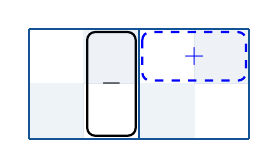
\begin{tikzpicture}[tableau, scale = .7]
        \gridLines{1}{2}
        \verticalDomino{1}{2}{-}
        \horizontalDominoMaybe{1}{3}{+}
        \fixedSquaresForGrid{1}{2}
      \end{tikzpicture}}}
      \quad\text{or}\quad
      \vcenter{\hbox{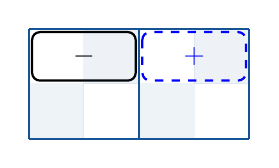
\begin{tikzpicture}[tableau, scale = .7]
        \gridLines{1}{2}
        \horizontalDomino{1}{1}{-}
        \horizontalDominoMaybe{1}{3}{+}
        \fixedSquaresForGrid{1}{2}
      \end{tikzpicture}}}
    \end{equation*}

    \item If the adjacent domino is vertical and has no sign, we're good to go.
    \begin{figure}[H]
      \centering
      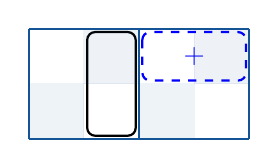
\begin{tikzpicture}[tableau, scale = .7]
        \gridLines{1}{2}
        \verticalDomino{1}{2}{ }
        \horizontalDominoMaybe{1}{3}{+}
        \fixedSquaresForGrid{1}{2}
      \end{tikzpicture}
    \end{figure}
    \item If the adjacent domino is horizontal and holds the same sign, we can't use this row.
    Let $r_0$ be the length of this row, let $r_1$ be the length of the next row, and let $r_2$ be the length of the row below that.
    \begin{itemize}
      \item If $r_0 = r_1$, then the next row also effectively has the same sign, and the domino can't be added there either.
      However, since the adjacent domino is horizontal, then the domino at the end of the next row is the top right end of a boxed inner cycle, and $r_2 < r_1$.
      So, we return the row two rows down from the current row as the place to try next.

      Here is an example.
      \begin{figure}[H]
        \centering
        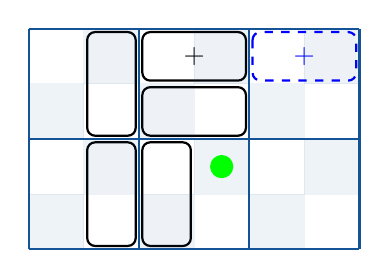
\begin{tikzpicture}[tableau, scale = .7]
          \gridLines{2}{3}
          \verticalDomino{1}{2}{ }
          \horizontalDomino{1}{3}{+}
          \horizontalDominoMaybe{1}{5}{+}
          \horizontalDomino{2}{3}{ }
          \verticalDomino{3}{2}{ }
          \verticalDomino{3}{3}{ }
          \fixedSquaresForGrid{2}{3}
          \greenCircle{3}{4}
        \end{tikzpicture}
      \end{figure}

      \item If $r_1 = r_0 - 1$, then the domino at the end of the next row is the top end of an unboxed inner cycle.
      \begin{itemize}
        \item If $r_2 < r_1$, then the next row ends in a horizontal domino and we can go straight to the row two rows down.
        \begin{figure}[H]
          \centering
          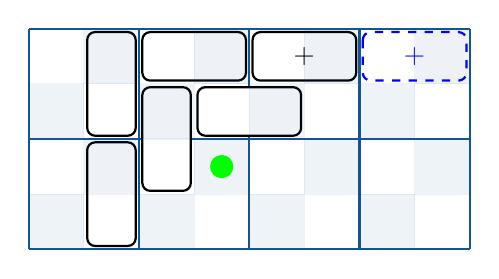
\begin{tikzpicture}[tableau, scale = .7]
            \gridLines{2}{4}
            \verticalDomino{1}{2}{ }
            \verticalDomino{3}{2}{ }
            \horizontalDomino{1}{3}{ }
            \horizontalDomino{1}{5}{+}
            \horizontalDominoMaybe{1}{7}{+}
            \verticalDomino{2}{3}{ }
            \horizontalDomino{2}{4}{ }
            \fixedSquaresForGrid{2}{4}
            \greenCircle{3}{4}
          \end{tikzpicture}
        \end{figure}
        \item Otherwise, the next row ends in a vertical domino, and we'll place our domino there.
        \begin{figure}[H]
          \centering
          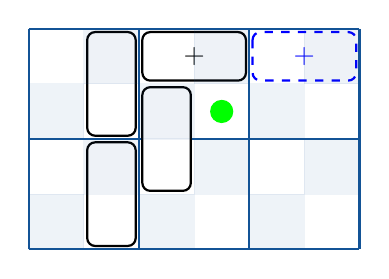
\begin{tikzpicture}[tableau, scale = .7]
            \gridLines{2}{3}
            \verticalDomino{1}{2}{ }
            \horizontalDomino{1}{3}{+}
            \horizontalDominoMaybe{1}{5}{+}
            \verticalDomino{2}{3}{ }
            \verticalDomino{3}{2}{ }
            \fixedSquaresForGrid{2}{3}
            \greenCircle{2}{4}
          \end{tikzpicture}
        \end{figure}
      \end{itemize}
      \item In all other cases (that is, $r_1 < r_0 - 1$), we'll try at the next row.
      \begin{figure}[H]
        \centering
        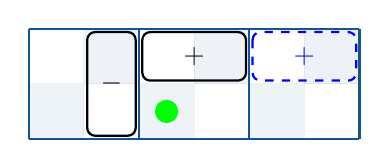
\begin{tikzpicture}[tableau, scale = .7]
          \gridLines{1}{3}
          \verticalDomino{1}{2}{-}
          \horizontalDomino{1}{3}{+}
          \horizontalDominoMaybe{1}{5}{+}
          \fixedSquaresForGrid{1}{3}
          \greenCircle{2}{3}
        \end{tikzpicture}
      \end{figure}
    \end{itemize}
    \item If the adjacent domino is horizontal and has no sign, then we can add at this row.
    It's possible that there are no paired dominoes at this level, and that the corner domino has the same sign in it.
    In this case, we can switch this sign down.
    (TODO, this needs proof.)
    The call to \texttt{makeSpaceFor()} will do the switch.
    \begin{figure}[H]
      \centering
      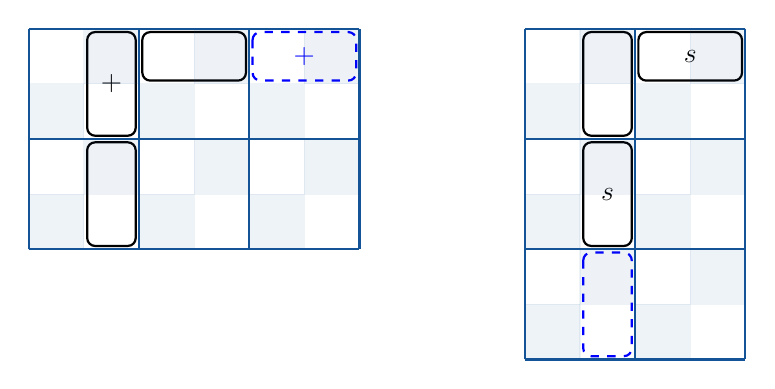
\begin{tikzpicture}[tableau, scale = .7]
        \gridLines{2}{3}
        \verticalDomino{1}{2}{+}
        \horizontalDomino{1}{3}{}
        \horizontalDominoMaybe{1}{5}{+}
        \verticalDomino{3}{2}{ }
        \fixedSquaresForGrid{2}{3}

        \gridLinesShift{3}{2}{9}
        \verticalDominoShift{1}{2}{ }{9}
        \horizontalDominoShift{1}{3}{s}{9}
        \verticalDominoShift{3}{2}{s}{9}
        \verticalDominoMaybeShift{5}{2}{ }{9}
        \fixedSquaresForGridShift{3}{2}{9}
      \end{tikzpicture}
    \end{figure}
    \item Finally, we have two cases where the adjacent domino is vertical and contains the same sign.
    We need to see if there is a blank domino in the column of the vertical domino which can be switched up.
    To do this, we search for a signed domino in the corresponding row of the dual sign tableau.
    The function used is \texttt{findSignInRowRight()}.
    \begin{itemize}
      \item If we do find a sign in the dual tableau's row, we call \linebreak \texttt{switchInRow()} (basically, focusing on the dual tableau) to move the sign up.
      Then we can add the original sign at this row.
      \begin{figure}[H]
        \centering
        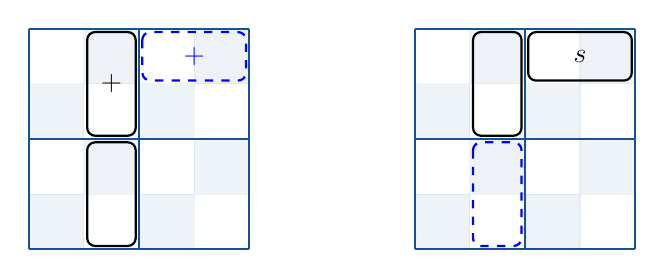
\begin{tikzpicture}[tableau, scale = .7]
          \gridLines{2}{2}
          \verticalDomino{1}{2}{+}
          \horizontalDominoMaybe{1}{3}{+}
          \verticalDomino{3}{2}{ }
          \fixedSquaresForGrid{2}{2}

          \gridLinesShift{2}{2}{7}
          \verticalDominoShift{1}{2}{ }{7}
          \horizontalDominoShift{1}{3}{s}{7}
          \verticalDominoMaybeShift{3}{2}{ }{7}
          \fixedSquaresForGridShift{2}{2}{7}
        \end{tikzpicture}
      \end{figure}
      Note, there may have been a relevant shape change from the call to \texttt{switchInRow()}.
      If so, we pass this information on by returning -1.

      We only need to know about a shape change which occurs right where we are putting the domino.
      This can happen if the vertical domino which we are next to is at the bottom of a cycle.
      In this case, when we swap it for a blank domino, we are putting a signed domino in the top of the corresponding cycle on the dual side.
      This may cause a shape change, as in the following example.
      \begin{figure}[H]
        \centering
        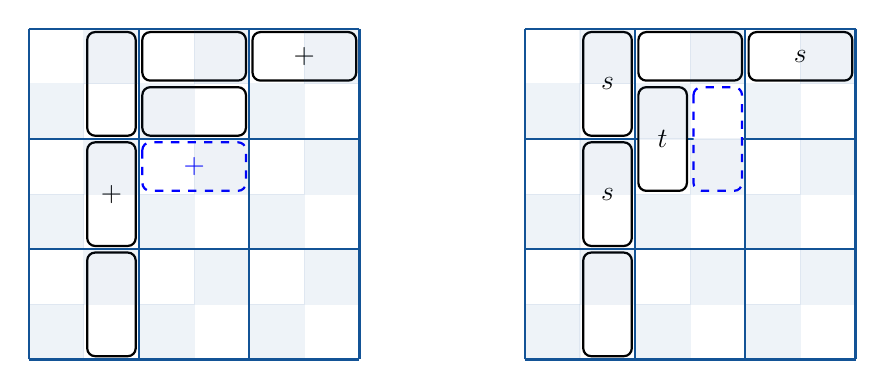
\begin{tikzpicture}[tableau, scale = .7]
          \gridLines{3}{3}
          \verticalDomino{1}{2}{ }
          \horizontalDomino{1}{3}{ }
          \horizontalDomino{1}{5}{+}
          \horizontalDomino{2}{3}{ }
          \verticalDomino{3}{2}{+}
          \horizontalDominoMaybe{3}{3}{+}
          \verticalDomino{5}{2}{ }
          \fixedSquaresForGrid{3}{3}

          \gridLinesShift{3}{3}{9}
          \verticalDominoShift{1}{2}{s}{9}
          \horizontalDominoShift{1}{3}{ }{9}
          \horizontalDominoShift{1}{5}{s}{9}
          \verticalDominoShift{3}{2}{s}{9}
          \verticalDominoShift{2}{3}{t}{9}
          \verticalDominoShift{5}{2}{ }{9}
          \verticalDominoMaybeShift{2}{4}{ }{9}
          \fixedSquaresForGridShift{3}{3}{9}
        \end{tikzpicture}
      \end{figure}
      goes to
      \begin{figure}[H]
        \centering
        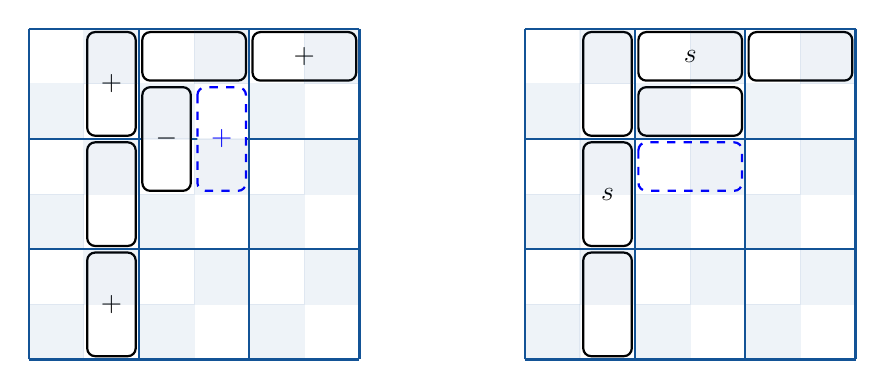
\begin{tikzpicture}[tableau, scale = .7]
          \gridLines{3}{3}
          \verticalDomino{1}{2}{+}
          \horizontalDomino{1}{3}{ }
          \horizontalDomino{1}{5}{+}
          \verticalDomino{2}{3}{-}
          \verticalDomino{3}{2}{ }
          \verticalDominoMaybe{2}{4}{+}
          \verticalDomino{5}{2}{+}
          \fixedSquaresForGrid{3}{3}

          \gridLinesShift{3}{3}{9}
          \verticalDominoShift{1}{2}{ }{9}
          \horizontalDominoShift{1}{3}{s}{9}
          \horizontalDominoShift{1}{5}{ }{9}
          \verticalDominoShift{3}{2}{s}{9}
          \horizontalDominoShift{2}{3}{ }{9}
          \verticalDominoShift{5}{2}{ }{9}
          \horizontalDominoMaybeShift{3}{3}{ }{9}
          \fixedSquaresForGridShift{3}{3}{9}
        \end{tikzpicture}
      \end{figure}
      \item If we do not find a sign in the dual tableau's row, then all the signs in the column are the same as the sign we are trying to add.
      So then, we try again at the row just below the column.
      \begin{figure}[H]
        \centering
        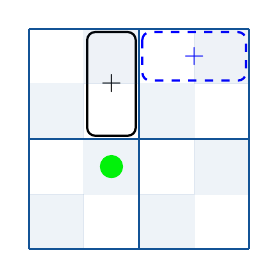
\begin{tikzpicture}[tableau, scale = .7]
          \gridLines{2}{2}
          \verticalDomino{1}{2}{+}
          \horizontalDominoMaybe{1}{3}{+}
          \greenCircle{3}{2}
          \fixedSquaresForGrid{2}{2}
        \end{tikzpicture}
      \end{figure}
    \end{itemize}
  \end{itemize}

  We return now to \texttt{addNumberSign()}
  We'll start with grid position $X$.
  Let's do the cases.
  Here, we assume that we have already called \linebreak \texttt{findRowToAddSignX()}, and that we are at a row where we can add the domino.
  \begin{itemize}
    \item The first case here is that we are extending an up cycle with a horizontal domino.
    In this case, we just put a horizontal domino with a $+$, starting at $(x, y)$.
    The dual sign domino is blank and is placed as a vertical domino starting in the square $(y, x + 1)$.
    \begin{figure}[H]
      \centering
      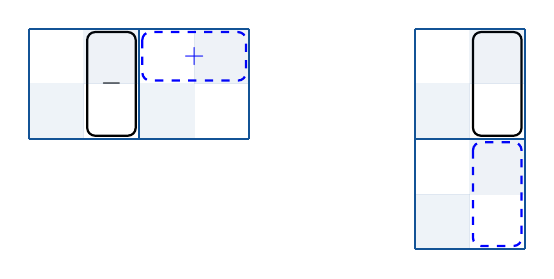
\begin{tikzpicture}[tableau, scale = .7]
        \gridLines{1}{2}
        \verticalDomino{1}{2}{-}
        \horizontalDominoMaybe{1}{3}{+}
        \fixedSquaresForGrid{1}{2}

        \gridLinesShift{2}{1}{7}
        \verticalDominoShift{1}{2}{ }{7}
        \verticalDominoMaybeShift{3}{2}{ }{7}
        \fixedSquaresForGridShift{2}{1}{7}
      \end{tikzpicture}
    \end{figure}

    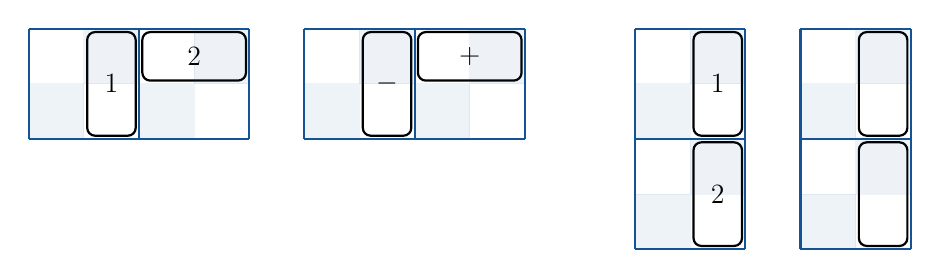
\begin{tikzpicture}[tableau, scale=.7]\gridLines{1}{2}\verticalDomino{1}{2}{1}\horizontalDomino{1}{3}{2}\fixedSquaresForGrid{1}{2}\gridLinesShift{1}{2}{5}\verticalDominoShift{1}{2}{-}{5}\horizontalDominoShift{1}{3}{+}{5}\fixedSquaresForGridShift{1}{2}{5}\gridLinesShift{2}{1}{11}\verticalDominoShift{1}{2}{1}{11}\verticalDominoShift{3}{2}{2}{11}\fixedSquaresForGridShift{2}{1}{11}\gridLinesShift{2}{1}{14}\verticalDominoShift{1}{2}{}{14}\verticalDominoShift{3}{2}{}{14}\fixedSquaresForGridShiftAlt{2}{1}{14}\end{tikzpicture}

    \item Next up is contracting a down cycle.
    The adjacent domino is then the bottom domino of the cycle which nests the cycle which you are contracting.
    First, here's a basic example:
    \begin{figure}[H]
      \centering
      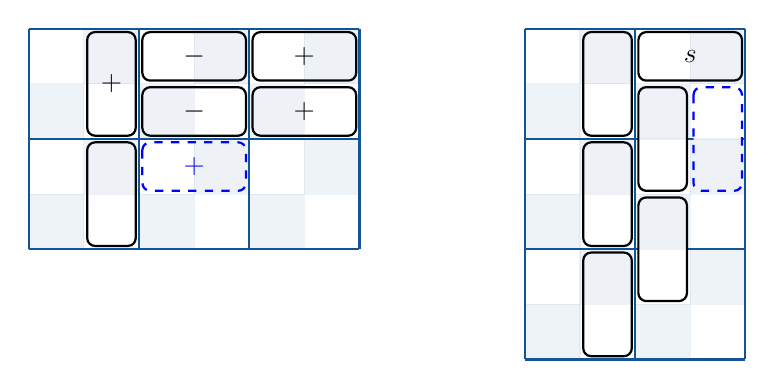
\begin{tikzpicture}[tableau, scale = .7]
        \gridLines{2}{3}
        \verticalDomino{1}{2}{+}
        \horizontalDomino{1}{3}{-}
        \horizontalDomino{2}{3}{-}
        \horizontalDomino{1}{5}{+}
        \horizontalDomino{2}{5}{+}
        \verticalDomino{3}{2}{ }
        \horizontalDominoMaybe{3}{3}{+}
        \fixedSquaresForGrid{2}{3}

        \gridLinesShift{3}{2}{9}
        \verticalDominoShift{1}{2}{ }{9}
        \horizontalDominoShift{1}{3}{s}{9}
        \verticalDominoShift{3}{2}{ }{9}
        \verticalDominoShift{2}{3}{ }{9}
        \verticalDominoShift{5}{2}{ }{9}
        \verticalDominoShift{4}{3}{ }{9}
        \verticalDominoMaybeShift{2}{4}{ }{9}
        \fixedSquaresForGridShift{3}{2}{9}
      \end{tikzpicture}
    \end{figure}
    There is a situation which we need to handle first.
    If the adjacent domino is blank, then we are putting a new sign in the bottom of the cycle in which the down cycle is nested.
    So, there's a call to \texttt{putSignInCycleBottom()}.
    Since we have not contracted the cycle yet, the adjacent domino is the cycle bottom.
    However, the added domino will be the new cycle bottom.
    So, we need to use $-$ as the sign to put into the cycle bottom when the adjacent domino is the cycle bottom.
    In our example:
    \begin{figure}[H]
      \centering
      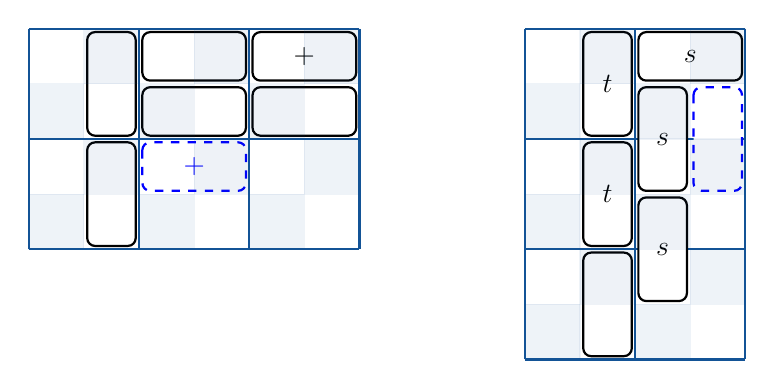
\begin{tikzpicture}[tableau, scale = .7]
        \gridLines{2}{3}
        \verticalDomino{1}{2}{ }
        \horizontalDomino{1}{3}{ }
        \horizontalDomino{2}{3}{ }
        \horizontalDomino{1}{5}{+}
        \horizontalDomino{2}{5}{ }
        \verticalDomino{3}{2}{ }
        \horizontalDominoMaybe{3}{3}{+}
        \fixedSquaresForGrid{2}{3}

        \gridLinesShift{3}{2}{9}
        \verticalDominoShift{1}{2}{t}{9}
        \horizontalDominoShift{1}{3}{s}{9}
        \verticalDominoShift{3}{2}{t}{9}
        \verticalDominoShift{2}{3}{s}{9}
        \verticalDominoShift{5}{2}{ }{9}
        \verticalDominoShift{4}{3}{s}{9}
        \verticalDominoMaybeShift{2}{4}{ }{9}
        \fixedSquaresForGridShift{3}{2}{9}
      \end{tikzpicture}
    \end{figure}

    We need to know that this will not change shape. \linebreak
    Now, \texttt{putSignInCycleBottom()} can change shape only when the nested cycle is unboxed.
    In our situation, the nested cycle starts out boxed.
    It will only be unboxed if its shape was changed by \linebreak \texttt{findRowToAddSignX()}.
    However, this shape change, if it happened, happened when taking $+$ out of the adjacent domino.
    So, the shape would only change back if we put $+$ in again.
    However, we are putting $-$ in, so the shape will not change back to boxed, if it is currently unboxed.

    Now we can place the domino.
    There are two cases, depending on whether or not there has been a shape change from \linebreak \texttt{findRowToAddSignX()}.
    \begin{itemize}
      \item If there is no shape change, we put a horizontal domino with a $+$, starting at $(x, y)$.
      The dual domino is vertical, at $(y, x)$.
      \item  If there has been a shape change, then the $(x, y)$ square is now occupied.
      We again put a horizontal domino with a $+$, but this time it starts at $(x + 1, y)$.
      The dual domino is vertical, at $(y, x + 1)$.
    \end{itemize}

    Finally, we need to box up the new domino, since we are contracting a cycle.
    We call \texttt{makeBox()} on the new domino, and on the corresponding domino in the dual sign tableau.
    In our main example:
    \begin{figure}[H]
      \centering
      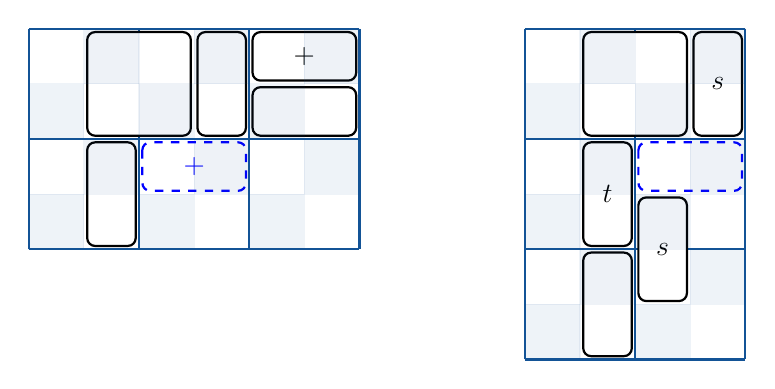
\begin{tikzpicture}[tableau, scale = .7]
        \gridLines{2}{3}
        \emptyBox{1}{2}
        \verticalDomino{1}{4}{ }
        \horizontalDomino{1}{5}{+}
        \horizontalDomino{2}{5}{ }
        \verticalDomino{3}{2}{ }
        \horizontalDominoMaybe{3}{3}{+}
        \fixedSquaresForGrid{2}{3}

        \gridLinesShift{3}{2}{9}
        \emptyBoxShift{1}{2}{9}
        \verticalDominoShift{1}{4}{s}{9}
        \verticalDominoShift{3}{2}{t}{9}
        \verticalDominoShift{5}{2}{ }{9}
        \verticalDominoShift{4}{3}{s}{9}
        \horizontalDominoMaybeShift{3}{3}{ }{9}
        \fixedSquaresForGridShift{3}{2}{9}
      \end{tikzpicture}
    \end{figure}

    \begin{figure}[H]
      \centering
      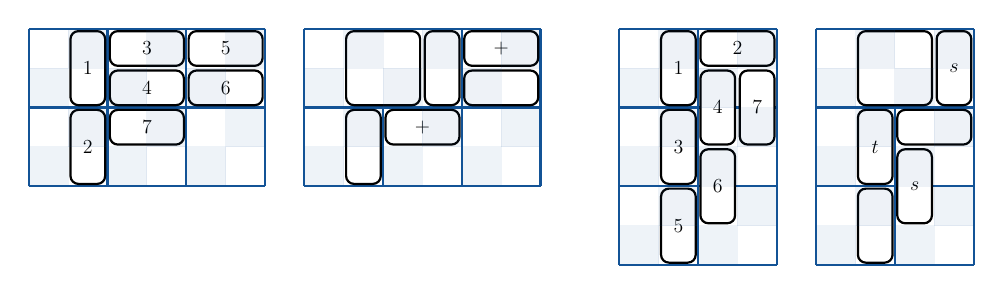
\begin{tikzpicture}[tableau, scale=.5]\gridLines{2}{3}\verticalDomino{1}{2}{1}\verticalDomino{3}{2}{2}\horizontalDomino{1}{3}{3}\horizontalDomino{2}{3}{4}\horizontalDomino{1}{5}{5}\horizontalDomino{2}{5}{6}\horizontalDomino{3}{3}{7}\fixedSquaresForGrid{2}{3}\gridLinesShift{2}{3}{7}\verticalDominoShift{3}{2}{}{7}\verticalDominoShift{1}{4}{}{7}\horizontalDominoShift{1}{5}{+}{7}\horizontalDominoShift{2}{5}{}{7}\horizontalDominoShift{3}{3}{+}{7}\emptyBoxShift{1}{2}{7}\fixedSquaresForGridShift{2}{3}{7}\gridLinesShift{3}{2}{15}\verticalDominoShift{1}{2}{1}{15}\horizontalDominoShift{1}{3}{2}{15}\verticalDominoShift{3}{2}{3}{15}\verticalDominoShift{2}{3}{4}{15}\verticalDominoShift{5}{2}{5}{15}\verticalDominoShift{4}{3}{6}{15}\verticalDominoShift{2}{4}{7}{15}\fixedSquaresForGridShift{3}{2}{15}\gridLinesShift{3}{2}{20}\verticalDominoShift{1}{4}{s}{20}\verticalDominoShift{3}{2}{t}{20}\verticalDominoShift{5}{2}{}{20}\verticalDominoShift{4}{3}{s}{20}\horizontalDominoShift{3}{3}{}{20}\emptyBoxShift{1}{2}{20}\fixedSquaresForGridShiftAlt{3}{2}{20}\end{tikzpicture}
    \end{figure}

    \item Here we are connecting two up cycles.
    We put a horizontal domino with a $+$, starting at $(x, y)$.
   The dual domino is vertical, at $(y - 1, x + 1)$.
   \begin{figure}[H]
     \centering
     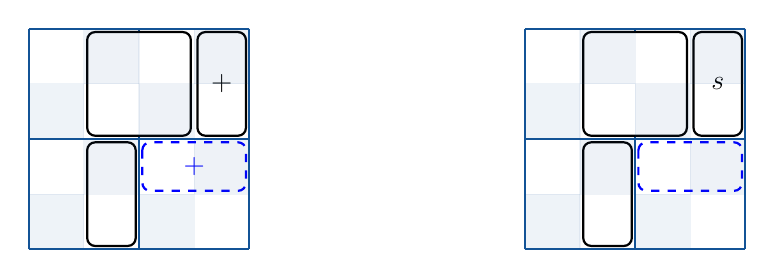
\begin{tikzpicture}[tableau, scale = .7]
       \gridLines{2}{2}
       \emptyBox{1}{2}
       \verticalDomino{1}{4}{+}
       \verticalDomino{3}{2}{ }
       \horizontalDominoMaybe{3}{3}{+}
       \fixedSquaresForGrid{2}{2}

       \gridLinesShift{2}{2}{9}
       \emptyBoxShift{1}{2}{9}
       \verticalDominoShift{1}{4}{s}{9}
       \verticalDominoShift{3}{2}{ }{9}
       \horizontalDominoMaybeShift{3}{3}{ }{9}
       \fixedSquaresForGridShift{2}{2}{9}
     \end{tikzpicture}
   \end{figure}

   \begin{figure}[H]
     \centering
     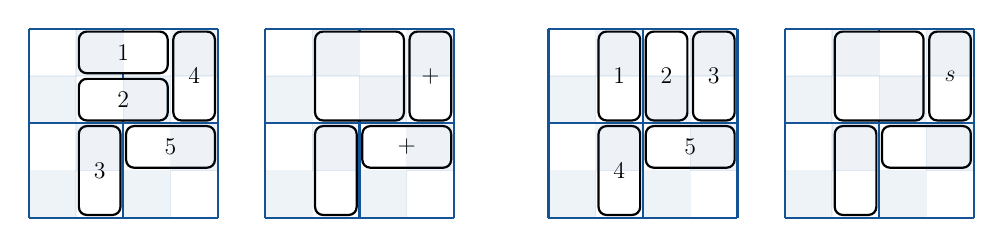
\begin{tikzpicture}[tableau, scale=.6]\gridLines{2}{2}\horizontalDomino{1}{2}{1}\horizontalDomino{2}{2}{2}\verticalDomino{3}{2}{3}\verticalDomino{1}{4}{4}\horizontalDomino{3}{3}{5}\fixedSquaresForGrid{2}{2}\gridLinesShift{2}{2}{5}\emptyBoxShift{1}{2}{5}\verticalDominoShift{3}{2}{}{5}\verticalDominoShift{1}{4}{+}{5}\horizontalDominoShift{3}{3}{+}{5}\fixedSquaresForGridShift{2}{2}{5}\gridLinesShift{2}{2}{11}\verticalDominoShift{1}{2}{1}{11}\verticalDominoShift{1}{3}{2}{11}\verticalDominoShift{1}{4}{3}{11}\verticalDominoShift{3}{2}{4}{11}\horizontalDominoShift{3}{3}{5}{11}\fixedSquaresForGridShift{2}{2}{11}\gridLinesShift{2}{2}{16}\emptyBoxShift{1}{2}{16}\verticalDominoShift{1}{4}{s}{16}\verticalDominoShift{3}{2}{}{16}\horizontalDominoShift{3}{3}{}{16}\fixedSquaresForGridShiftAlt{2}{2}{16}\end{tikzpicture}
  \end{figure}

   \item Here we are closing a down cycle.
   There might be a shape change.
   \begin{itemize}
     \item If there is no shape change, we put a horizontal domino with a $+$, starting at $(x, y)$.
     The dual domino is vertical, at $(y, x)$.
     \begin{figure}[H]
       \centering
       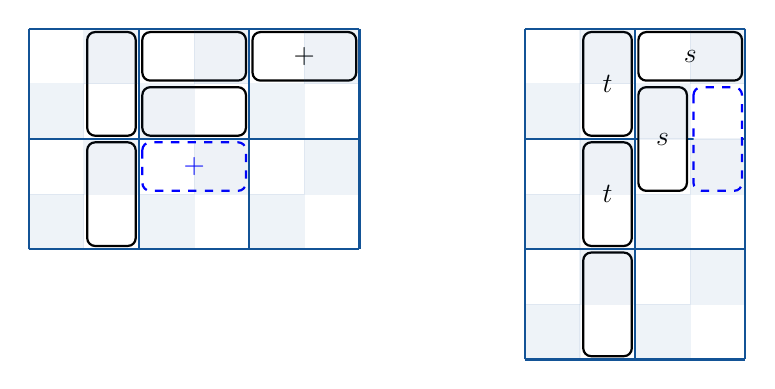
\begin{tikzpicture}[tableau, scale = .7]
         \gridLines{2}{3}
         \verticalDomino{1}{2}{ }
         \horizontalDomino{1}{3}{ }
         \horizontalDomino{2}{3}{ }
         \horizontalDomino{1}{5}{+}
         \verticalDomino{3}{2}{ }
         \horizontalDominoMaybe{3}{3}{+}
         \fixedSquaresForGrid{2}{3}

         \gridLinesShift{3}{2}{9}
         \verticalDominoShift{1}{2}{t}{9}
         \horizontalDominoShift{1}{3}{s}{9}
         \verticalDominoShift{3}{2}{t}{9}
         \verticalDominoShift{2}{3}{s}{9}
         \verticalDominoShift{5}{2}{ }{9}
         \verticalDominoMaybeShift{2}{4}{ }{9}
         \fixedSquaresForGridShift{3}{2}{9}
       \end{tikzpicture}
     \end{figure}
     \item  If there has been a shape change, then we put a vertical domino with a $+$, starting at $(x + 1, y - 1)$.
     The dual domino is vertical, at $(y - 1, x + 1)$.
   \end{itemize}
   We need to box up the new domino, since we are closing a cycle.
   We call \texttt{makeBox()} on the new domino, and on the corresponding domino in the dual sign tableau.

   The newly-added domino is now in a level I cycle with the domino whose fixed square is two squares above the domino's fixed square.
   Note, this domino cannot have the opposite sign.
   It is either blank or has the same sign.
   (TODO, find and add the argument.)
   If it is blank, in principle we may be able to move the newly-added domino up.
   However, I don't think this is possible, and I have commented out the code to check.
   This needs proof.
   % TODO, I think this is unnecessary.
   % We call \texttt{switchAfterAddX()} to check this and do this if necessary.
   \begin{figure}[H]
     \centering
     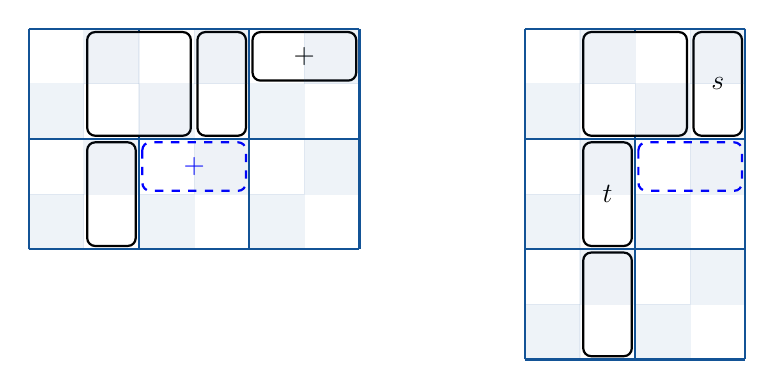
\begin{tikzpicture}[tableau, scale = .7]
       \gridLines{2}{3}
       \emptyBox{1}{2}
       \verticalDomino{1}{4}{ }
       \horizontalDomino{1}{5}{+}
       \verticalDomino{3}{2}{ }
       \horizontalDominoMaybe{3}{3}{+}
       \fixedSquaresForGrid{2}{3}

       \gridLinesShift{3}{2}{9}
       \emptyBoxShift{1}{2}{9}
       \verticalDominoShift{1}{4}{s}{9}
       \verticalDominoShift{3}{2}{t}{9}
       \verticalDominoShift{5}{2}{ }{9}
       \horizontalDominoMaybeShift{3}{3}{ }{9}
       \fixedSquaresForGridShift{3}{2}{9}
     \end{tikzpicture}
   \end{figure}

   \begin{figure}[H]
     \centering
     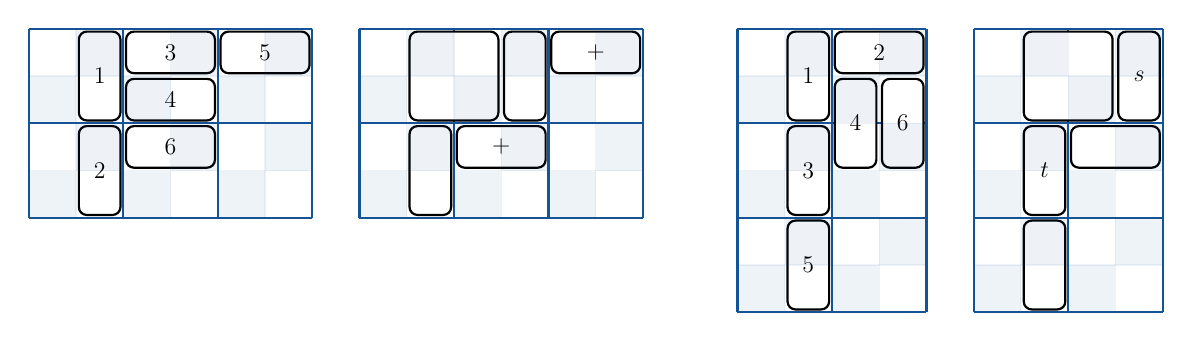
\begin{tikzpicture}[tableau, scale=.6]\gridLines{2}{3}\verticalDomino{1}{2}{1}\verticalDomino{3}{2}{2}\horizontalDomino{1}{3}{3}\horizontalDomino{2}{3}{4}\horizontalDomino{1}{5}{5}\horizontalDomino{3}{3}{6}\fixedSquaresForGrid{2}{3}\gridLinesShift{2}{3}{7}\verticalDominoShift{3}{2}{}{7}\verticalDominoShift{1}{4}{}{7}\horizontalDominoShift{1}{5}{+}{7}\horizontalDominoShift{3}{3}{+}{7}\emptyBoxShift{1}{2}{7}\fixedSquaresForGridShift{2}{3}{7}\gridLinesShift{3}{2}{15}\verticalDominoShift{1}{2}{1}{15}\horizontalDominoShift{1}{3}{2}{15}\verticalDominoShift{3}{2}{3}{15}\verticalDominoShift{2}{3}{4}{15}\verticalDominoShift{5}{2}{5}{15}\verticalDominoShift{2}{4}{6}{15}\fixedSquaresForGridShift{3}{2}{15}\gridLinesShift{3}{2}{20}\verticalDominoShift{1}{4}{s}{20}\verticalDominoShift{3}{2}{t}{20}\verticalDominoShift{5}{2}{}{20}\horizontalDominoShift{3}{3}{}{20}\emptyBoxShift{1}{2}{20}\fixedSquaresForGridShiftAlt{3}{2}{20}
     \end{tikzpicture}
  \end{figure}

   Now we return to our shape change example from \linebreak  \texttt{findRowToAddSignX()}.
   We have
   \begin{figure}[H]
     \centering
     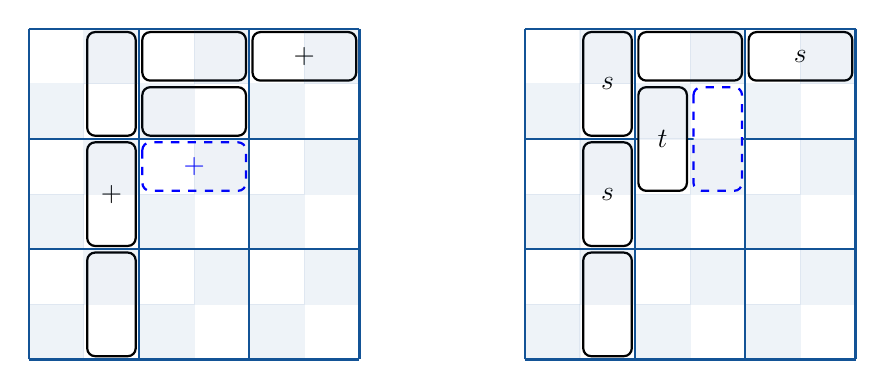
\begin{tikzpicture}[tableau, scale = .7]
       \gridLines{3}{3}
       \verticalDomino{1}{2}{ }
       \horizontalDomino{1}{3}{ }
       \horizontalDomino{1}{5}{+}
       \horizontalDomino{2}{3}{ }
       \verticalDomino{3}{2}{+}
       \horizontalDominoMaybe{3}{3}{+}
       \verticalDomino{5}{2}{ }
       \fixedSquaresForGrid{3}{3}

       \gridLinesShift{3}{3}{9}
       \verticalDominoShift{1}{2}{s}{9}
       \horizontalDominoShift{1}{3}{ }{9}
       \horizontalDominoShift{1}{5}{s}{9}
       \verticalDominoShift{3}{2}{s}{9}
       \verticalDominoShift{2}{3}{t}{9}
       \verticalDominoShift{5}{2}{ }{9}
       \verticalDominoMaybeShift{2}{4}{ }{9}
       \fixedSquaresForGridShift{3}{3}{9}
     \end{tikzpicture}
   \end{figure}
   goes to
   \begin{figure}[H]
     \centering
     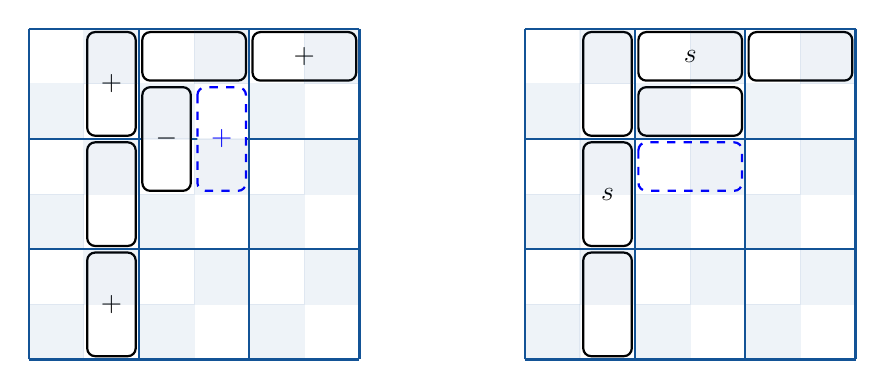
\begin{tikzpicture}[tableau, scale = .7]
       \gridLines{3}{3}
       \verticalDomino{1}{2}{+}
       \horizontalDomino{1}{3}{ }
       \horizontalDomino{1}{5}{+}
       \verticalDomino{2}{3}{-}
       \verticalDomino{3}{2}{ }
       \verticalDominoMaybe{2}{4}{+}
       \verticalDomino{5}{2}{+}
       \fixedSquaresForGrid{3}{3}

       \gridLinesShift{3}{3}{9}
       \verticalDominoShift{1}{2}{ }{9}
       \horizontalDominoShift{1}{3}{s}{9}
       \horizontalDominoShift{1}{5}{ }{9}
       \verticalDominoShift{3}{2}{s}{9}
       \horizontalDominoShift{2}{3}{ }{9}
       \verticalDominoShift{5}{2}{ }{9}
       \horizontalDominoMaybeShift{3}{3}{ }{9}
       \fixedSquaresForGridShift{3}{3}{9}
     \end{tikzpicture}
   \end{figure}

   and finally, we make the box:
   \begin{figure}[H]
     \centering
     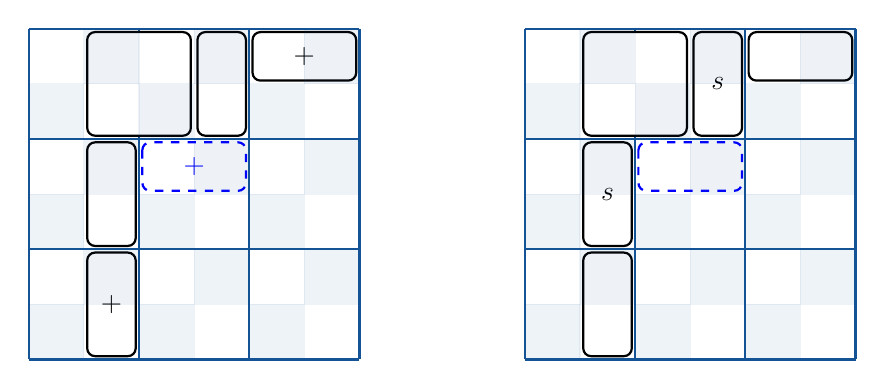
\begin{tikzpicture}[tableau, scale = .7]
       \gridLines{3}{3}
       \emptyBox{1}{2}
       \verticalDomino{1}{4}{ }
       \horizontalDomino{1}{5}{+}
       \verticalDomino{3}{2}{ }
       \horizontalDominoMaybe{3}{3}{+}
       \verticalDomino{5}{2}{+}
       \fixedSquaresForGrid{3}{3}

       \gridLinesShift{3}{3}{9}
       \emptyBoxShift{1}{2}{9}
       \verticalDominoShift{1}{4}{s}{9}
       \horizontalDominoShift{1}{5}{ }{9}
       \verticalDominoShift{3}{2}{s}{9}
       \verticalDominoShift{5}{2}{ }{9}
       \horizontalDominoMaybeShift{3}{3}{ }{9}
       \fixedSquaresForGridShift{3}{3}{9}
     \end{tikzpicture}
   \end{figure}

   Since we're closing a cycle, the sign tableaux really don't show the difference between the ordinary case and the shape change case.
   However, the number tableaux will show the difference.
   In the shape change case, the number domino is not in the same position as the sign domino, on the $+, -$ side.

   \bigskip

   \begin{figure}[H]
     \centering
     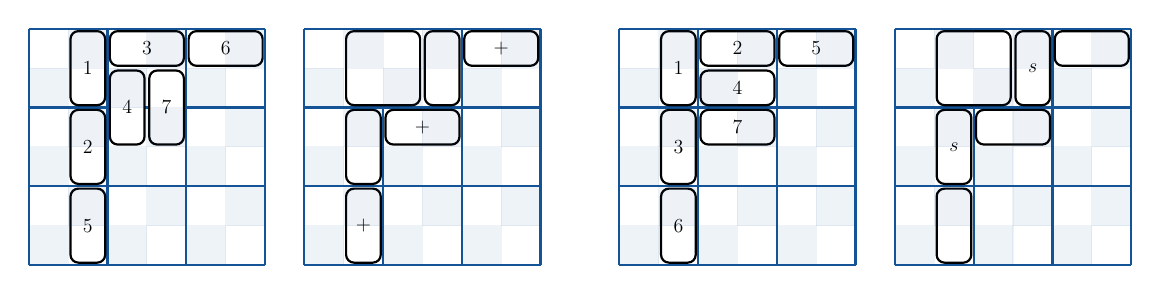
\begin{tikzpicture}[tableau, scale=.5]\gridLines{3}{3}\verticalDomino{1}{2}{1}\verticalDomino{3}{2}{2}\horizontalDomino{1}{3}{3}\verticalDomino{2}{3}{4}\verticalDomino{5}{2}{5}\horizontalDomino{1}{5}{6}\verticalDomino{2}{4}{7}\fixedSquaresForGrid{3}{3}\gridLinesShift{3}{3}{7}\verticalDominoShift{3}{2}{}{7}\verticalDominoShift{1}{4}{}{7}\verticalDominoShift{5}{2}{+}{7}\horizontalDominoShift{1}{5}{+}{7}\horizontalDominoShift{3}{3}{+}{7}\emptyBoxShift{1}{2}{7}\fixedSquaresForGridShift{3}{3}{7}\gridLinesShift{3}{3}{15}\verticalDominoShift{1}{2}{1}{15}\horizontalDominoShift{1}{3}{2}{15}\verticalDominoShift{3}{2}{3}{15}\horizontalDominoShift{2}{3}{4}{15}\horizontalDominoShift{1}{5}{5}{15}\verticalDominoShift{5}{2}{6}{15}\horizontalDominoShift{3}{3}{7}{15}\fixedSquaresForGridShift{3}{3}{15}\gridLinesShift{3}{3}{22}\verticalDominoShift{1}{4}{s}{22}\verticalDominoShift{3}{2}{s}{22}\horizontalDominoShift{1}{5}{}{22}\verticalDominoShift{5}{2}{}{22}\horizontalDominoShift{3}{3}{}{22}\emptyBoxShift{1}{2}{22}\fixedSquaresForGridShiftAlt{3}{3}{22}\end{tikzpicture}
  \end{figure}

   \item In this case, we are connecting an up and a down cycle at the top of the down cycle.
   This is handled by \texttt{joinTwoCycles()}.

   \item In this case, we are connecting an up and a down cycle at the bottom of the down cycle.
   This is handled by \texttt{joinTwoCycles()}.
  \end{itemize}

  Now, let's do the cases for grid position $Y$.
  We're looking to add at position $(x, y)$.
  If $y \neq 0$, let $rMinus$ be the length of the row $y - 1$.
  If $x \neq 0$, let $rPlus$ be the length of the row $y + 1$.
  The cases depend on whether or not the row above is longer than this row, that is, whether or not $rMinus > x + 1$, and on whether or not the row below has its maximum possible length, that is, whether or not $rPlus = x$.
  \begin{itemize}
    \item Here $x \neq 0$ and $rPlus < x$.
    In this case, we are right next to an unboxed cycle which ends here.
    These two cases mirror two of the cases where the grid square is $X$.
    That is, we first need to call \texttt{findRowToAddSignX()} to see if we can add the + sign at this level.
    If not, we go below.
    If we can add at this level, there are two cases.
    \begin{itemize}
      \item Here $y = 0$ or $rMinus > x + 1$.
      So, we we are contracting an unboxed cycle.
      \begin{figure}[H]
        \centering
        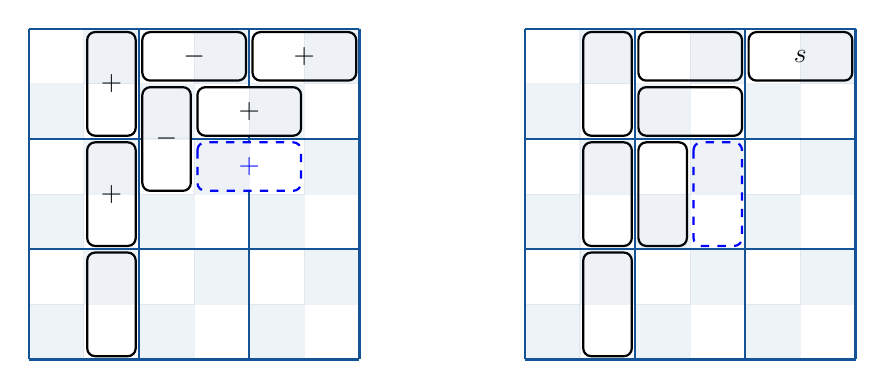
\begin{tikzpicture}[tableau, scale = .7]
          \gridLines{3}{3}
          \verticalDomino{1}{2}{+}
          \horizontalDomino{1}{3}{-}
          \horizontalDomino{1}{5}{+}
          \verticalDomino{3}{2}{+}
          \verticalDomino{2}{3}{-}
          \horizontalDomino{2}{4}{+}
          \horizontalDominoMaybe{3}{4}{+}
          \verticalDomino{5}{2}{ }
          \fixedSquaresForGrid{3}{3}

          \gridLinesShift{3}{3}{9}
          \verticalDominoShift{1}{2}{ }{9}
          \horizontalDominoShift{1}{3}{ }{9}
          \horizontalDominoShift{1}{5}{s}{9}
          \verticalDominoShift{3}{2}{ }{9}
          \horizontalDominoShift{2}{3}{ }{9}
          \verticalDominoShift{5}{2}{ }{9}
          \verticalDominoShift{3}{3}{ }{9}
          \verticalDominoMaybeShift{3}{4}{ }{9}
          \fixedSquaresForGridShift{3}{3}{9}
        \end{tikzpicture}
      \end{figure}
      There can't be a shape change from the call to \texttt{findRowToAddSignX()}, because we are adding the sign on the dual side, to the cycle top, and that can only make a change when the cycle is unboxed.
      However, the cycle is boxed on the dual side.
      The next step in this example is:
      \begin{figure}[H]
        \centering
        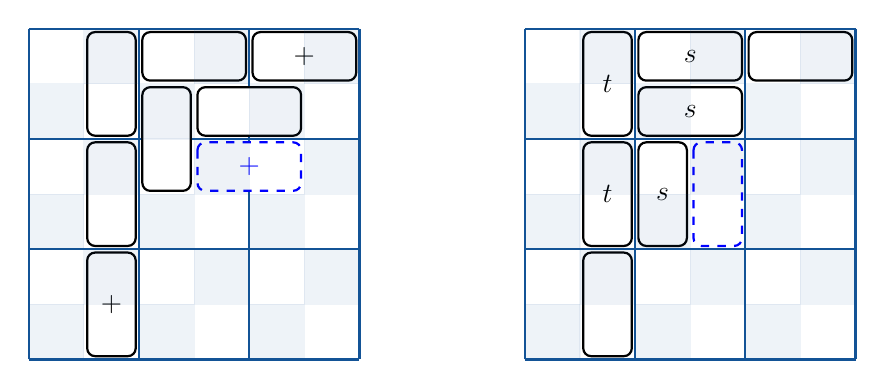
\begin{tikzpicture}[tableau, scale = .7]
          \gridLines{3}{3}
          \verticalDomino{1}{2}{ }
          \horizontalDomino{1}{3}{ }
          \horizontalDomino{1}{5}{+}
          \verticalDomino{3}{2}{ }
          \verticalDomino{2}{3}{ }
          \horizontalDomino{2}{4}{ }
          \horizontalDominoMaybe{3}{4}{+}
          \verticalDomino{5}{2}{+}
          \fixedSquaresForGrid{3}{3}

          \gridLinesShift{3}{3}{9}
          \verticalDominoShift{1}{2}{t}{9}
          \horizontalDominoShift{1}{3}{s}{9}
          \horizontalDominoShift{1}{5}{ }{9}
          \verticalDominoShift{3}{2}{t}{9}
          \horizontalDominoShift{2}{3}{s}{9}
          \verticalDominoShift{5}{2}{ }{9}
          \verticalDominoShift{3}{3}{s}{9}
          \verticalDominoMaybeShift{3}{4}{ }{9}
          \fixedSquaresForGridShift{3}{3}{9}
        \end{tikzpicture}
      \end{figure}
      Next, we put the numbered dominoes into the number tableaux, in the same blue positions.
      Now, let's box up the sign tableaux.
      \begin{figure}[H]
        \centering
        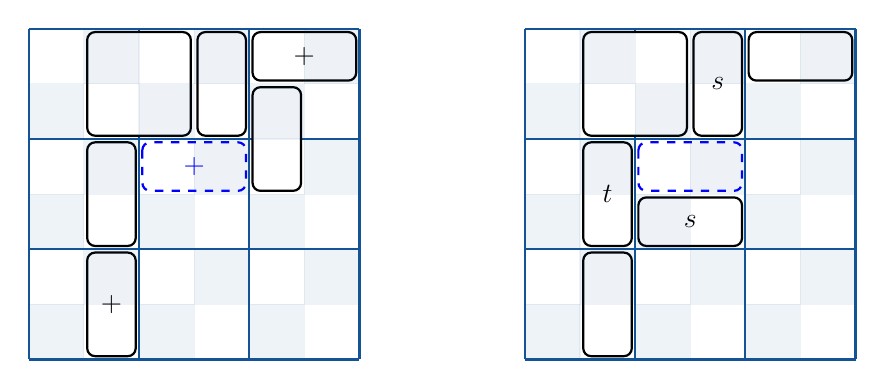
\begin{tikzpicture}[tableau, scale = .7]
          \gridLines{3}{3}
          \emptyBox{1}{2}
          \verticalDomino{1}{4}{ }
          \horizontalDomino{1}{5}{+}
          \verticalDomino{3}{2}{ }
          \verticalDomino{2}{5}{ }
          \horizontalDominoMaybe{3}{3}{+}
          \verticalDomino{5}{2}{+}
          \fixedSquaresForGrid{3}{3}

          \gridLinesShift{3}{3}{9}
          \emptyBoxShift{1}{2}{9}
          \verticalDominoShift{1}{4}{s}{9}
          \horizontalDominoShift{1}{5}{ }{9}
          \verticalDominoShift{3}{2}{t}{9}
          \verticalDominoShift{5}{2}{ }{9}
          \horizontalDominoShift{4}{3}{s}{9}
          \horizontalDominoMaybeShift{3}{3}{ }{9}
          \fixedSquaresForGridShift{3}{3}{9}
        \end{tikzpicture}
      \end{figure}

      Okay, last step.  The added domino is now in the bottom of the contracted cycle.
      We need to put that sign in the cycle bottom.
      As in this example, this may cause a shape change.
      \begin{figure}[H]
        \centering
        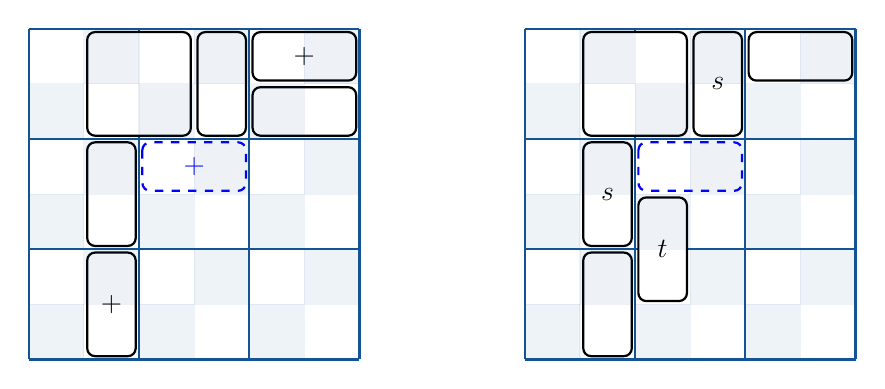
\begin{tikzpicture}[tableau, scale = .7]
          \gridLines{3}{3}
          \emptyBox{1}{2}
          \verticalDomino{1}{4}{ }
          \horizontalDomino{1}{5}{+}
          \verticalDomino{3}{2}{ }
          \horizontalDomino{2}{5}{ }
          \horizontalDominoMaybe{3}{3}{+}
          \verticalDomino{5}{2}{+}
          \fixedSquaresForGrid{3}{3}

          \gridLinesShift{3}{3}{9}
          \emptyBoxShift{1}{2}{9}
          \verticalDominoShift{1}{4}{s}{9}
          \horizontalDominoShift{1}{5}{ }{9}
          \verticalDominoShift{3}{2}{s}{9}
          \verticalDominoShift{5}{2}{ }{9}
          \verticalDominoShift{4}{3}{t}{9}
          \horizontalDominoMaybeShift{3}{3}{ }{9}
          \fixedSquaresForGridShift{3}{3}{9}
        \end{tikzpicture}
      \end{figure}

      \begin{figure}[H]
        \centering
        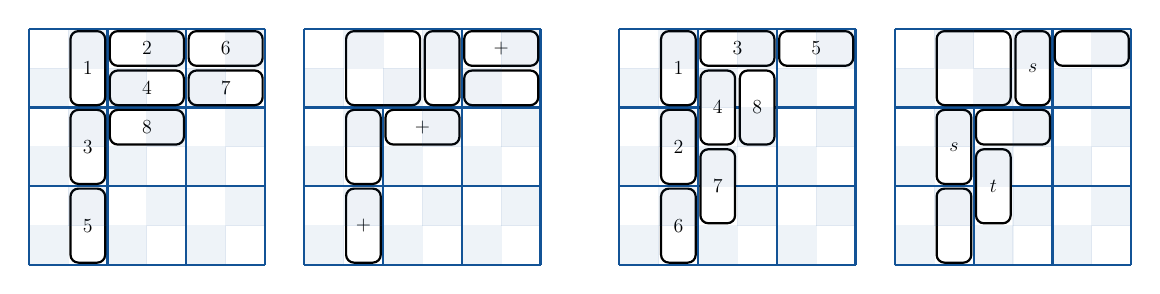
\begin{tikzpicture}[tableau, scale=.5]\gridLines{3}{3}\verticalDomino{1}{2}{1}\horizontalDomino{1}{3}{2}\verticalDomino{3}{2}{3}\horizontalDomino{2}{3}{4}\verticalDomino{5}{2}{5}\horizontalDomino{1}{5}{6}\horizontalDomino{2}{5}{7}\horizontalDomino{3}{3}{8}\fixedSquaresForGrid{3}{3}\gridLinesShift{3}{3}{7}\verticalDominoShift{1}{4}{}{7}\verticalDominoShift{3}{2}{}{7}\verticalDominoShift{5}{2}{+}{7}\horizontalDominoShift{1}{5}{+}{7}\horizontalDominoShift{2}{5}{}{7}\horizontalDominoShift{3}{3}{+}{7}\emptyBoxShift{1}{2}{7}\fixedSquaresForGridShift{3}{3}{7}\gridLinesShift{3}{3}{15}\verticalDominoShift{1}{2}{1}{15}\verticalDominoShift{3}{2}{2}{15}\horizontalDominoShift{1}{3}{3}{15}\verticalDominoShift{2}{3}{4}{15}\horizontalDominoShift{1}{5}{5}{15}\verticalDominoShift{5}{2}{6}{15}\verticalDominoShift{4}{3}{7}{15}\verticalDominoShift{2}{4}{8}{15}\fixedSquaresForGridShift{3}{3}{15}\gridLinesShift{3}{3}{22}\verticalDominoShift{3}{2}{s}{22}\verticalDominoShift{1}{4}{s}{22}\horizontalDominoShift{1}{5}{}{22}\verticalDominoShift{5}{2}{}{22}\verticalDominoShift{4}{3}{t}{22}\horizontalDominoShift{3}{3}{}{22}\emptyBoxShift{1}{2}{22}\fixedSquaresForGridShiftAlt{3}{3}{22}\end{tikzpicture}
      \end{figure}


      Here's an example with no shape change at the end.

      \begin{figure}[H]
        \centering
        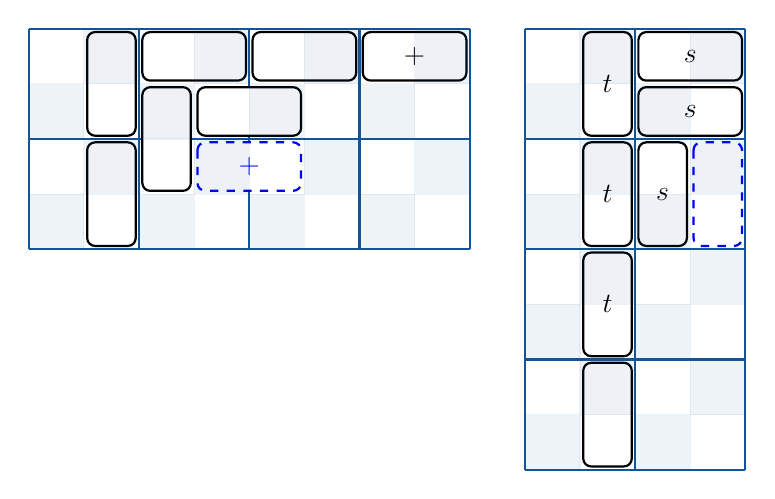
\begin{tikzpicture}[tableau, scale = .7]
          \gridLines{2}{4}
          \verticalDomino{1}{2}{ }
          \horizontalDomino{1}{3}{ }
          \horizontalDomino{1}{5}{ }
          \horizontalDomino{1}{7}{+}
          \verticalDomino{2}{3}{ }
          \horizontalDomino{2}{4}{ }
          \verticalDomino{3}{2}{ }
          \horizontalDominoMaybe{3}{4}{+}
          \fixedSquaresForGrid{2}{4}

          \gridLinesShift{4}{2}{9}
          \verticalDominoShift{1}{2}{t}{9}
          \horizontalDominoShift{1}{3}{s}{9}
          \verticalDominoShift{3}{2}{t}{9}
          \horizontalDominoShift{2}{3}{s}{9}
          \verticalDominoShift{5}{2}{t}{9}
          \verticalDominoShift{3}{3}{s}{9}
          \verticalDominoShift{7}{2}{ }{9}
          \verticalDominoMaybeShift{3}{4}{ }{9}
          \fixedSquaresForGridShift{4}{2}{9}
        \end{tikzpicture}
      \end{figure}
      The final result is:

      \bigskip

      \begin{figure}[H]
        \centering
        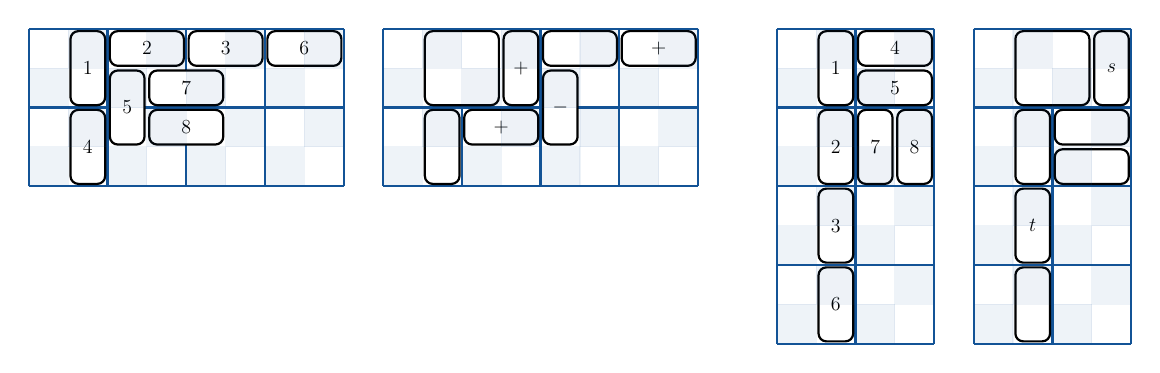
\begin{tikzpicture}[tableau, scale=.5]\gridLines{2}{4}\verticalDomino{1}{2}{1}\horizontalDomino{1}{3}{2}\horizontalDomino{1}{5}{3}\verticalDomino{3}{2}{4}\verticalDomino{2}{3}{5}\horizontalDomino{1}{7}{6}\horizontalDomino{2}{4}{7}\horizontalDomino{3}{4}{8}\fixedSquaresForGrid{2}{4}\gridLinesShift{2}{4}{9}\verticalDominoShift{1}{4}{+}{9}\horizontalDominoShift{1}{5}{}{9}\verticalDominoShift{3}{2}{}{9}\horizontalDominoShift{1}{7}{+}{9}\verticalDominoShift{2}{5}{-}{9}\horizontalDominoShift{3}{3}{+}{9}\emptyBoxShift{1}{2}{9}\fixedSquaresForGridShift{2}{4}{9}\gridLinesShift{4}{2}{19}\verticalDominoShift{1}{2}{1}{19}\verticalDominoShift{3}{2}{2}{19}\verticalDominoShift{5}{2}{3}{19}\horizontalDominoShift{1}{3}{4}{19}\horizontalDominoShift{2}{3}{5}{19}\verticalDominoShift{7}{2}{6}{19}\verticalDominoShift{3}{3}{7}{19}\verticalDominoShift{3}{4}{8}{19}\fixedSquaresForGridShift{4}{2}{19}\gridLinesShift{4}{2}{24}\verticalDominoShift{3}{2}{}{24}\verticalDominoShift{5}{2}{t}{24}\verticalDominoShift{1}{4}{s}{24}\verticalDominoShift{7}{2}{}{24}\horizontalDominoShift{4}{3}{}{24}\horizontalDominoShift{3}{3}{}{24}\emptyBoxShift{1}{2}{24}\fixedSquaresForGridShiftAlt{4}{2}{24}\end{tikzpicture}
      \end{figure}
      \item Here $y > 0$ and $rMinus = x + 1$.
      So, we are connecting the unboxed cycle to a nested up cycle.
      \begin{figure}[H]
        \centering
        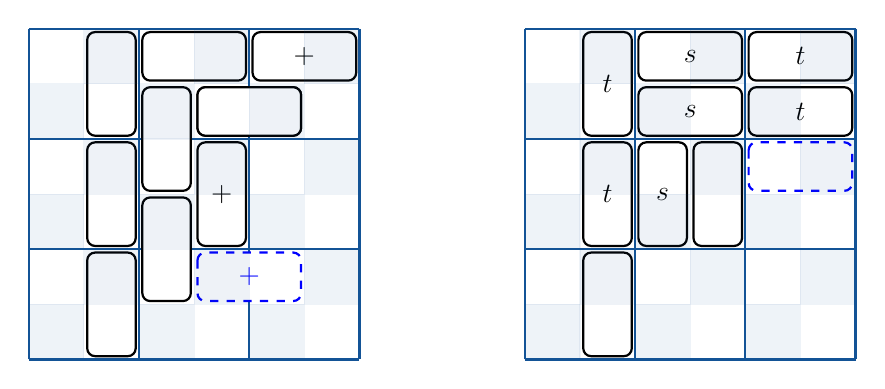
\begin{tikzpicture}[tableau, scale = .7]
          \gridLines{3}{3}
          \verticalDomino{1}{2}{ }
          \horizontalDomino{1}{3}{ }
          \horizontalDomino{1}{5}{+}
          \verticalDomino{2}{3}{ }
          \horizontalDomino{2}{4}{ }
          \verticalDomino{3}{2}{ }
          \verticalDomino{4}{3}{ }
          \horizontalDomino{2}{4}{ }
          \verticalDomino{3}{4}{+}
          \horizontalDominoMaybe{5}{4}{+}
          \verticalDomino{5}{2}{ }
          \fixedSquaresForGrid{3}{3}

          \gridLinesShift{3}{3}{9}
          \verticalDominoShift{1}{2}{t}{9}
          \horizontalDominoShift{1}{3}{s}{9}
          \horizontalDominoShift{1}{5}{t}{9}
          \verticalDominoShift{3}{2}{t}{9}
          \horizontalDominoShift{2}{3}{s}{9}
          \horizontalDominoShift{2}{5}{t}{9}
          \verticalDominoShift{5}{2}{ }{9}
          \verticalDominoShift{3}{3}{s}{9}
          \verticalDominoShift{3}{4}{ }{9}
          \horizontalDominoMaybeShift{3}{5}{ }{9}
          \fixedSquaresForGridShift{3}{3}{9}
        \end{tikzpicture}
      \end{figure}
      For now, we'll just reference \texttt{joinTwoCycles()}.
    \end{itemize}
    \item Here $x = 0$ or $rPlus = x$.
    Again, we split into the two situations.
    \begin{itemize}
      \item Here $y = 0$ or $rMinus > x + 1$.
      This is the situation with an empty tableau, for example.
      We are making a new cycle.
      \begin{figure}[H]
        \centering
        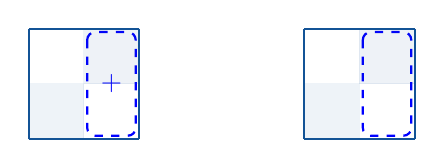
\begin{tikzpicture}[tableau, scale = .7]
          \gridLines{1}{1}
          \verticalDominoMaybe{1}{2}{+}
          \fixedSquaresForGrid{1}{1}

          \gridLinesShift{1}{1}{5}
          \verticalDominoMaybeShift{1}{2}{ }{5}
          \fixedSquaresForGridShift{1}{1}{5}
        \end{tikzpicture}
      \end{figure}

      \begin{figure}[H]
        \centering
        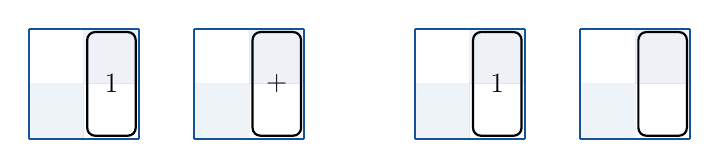
\begin{tikzpicture}[tableau, scale=.7]\gridLines{1}{1}\verticalDomino{1}{2}{1}\fixedSquaresForGrid{1}{1}\gridLinesShift{1}{1}{3}\verticalDominoShift{1}{2}{+}{3}\fixedSquaresForGridShift{1}{1}{3}\gridLinesShift{1}{1}{7}\verticalDominoShift{1}{2}{1}{7}\fixedSquaresForGridShift{1}{1}{7}\gridLinesShift{1}{1}{10}\verticalDominoShift{1}{2}{}{10}\fixedSquaresForGridShiftAlt{1}{1}{10}\end{tikzpicture}
      \end{figure}
      \item Here $y > 0$ and $rMinus = x + 1$.
      There are two cases
      \begin{itemize}
        \item Here we are extending an up cycle by putting another domino in its bottom:
        \begin{figure}[H]
          \centering
          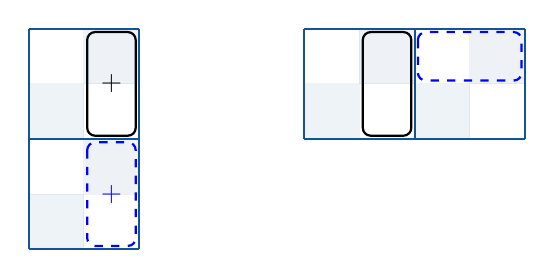
\begin{tikzpicture}[tableau, scale = .7]
            \gridLines{2}{1}
            \verticalDomino{1}{2}{+}
            \verticalDominoMaybe{3}{2}{+}
            \fixedSquaresForGrid{2}{1}

            \gridLinesShift{1}{2}{5}
            \verticalDominoShift{1}{2}{ }{5}
            \horizontalDominoMaybeShift{1}{3}{ }{5}
            \fixedSquaresForGridShift{1}{2}{5}
          \end{tikzpicture}
        \end{figure}

        \begin{figure}[H]
          \centering
          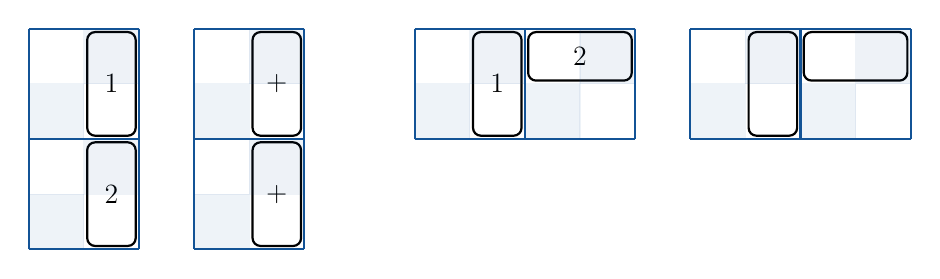
\begin{tikzpicture}[tableau, scale=.7]\gridLines{2}{1}\verticalDomino{1}{2}{1}\verticalDomino{3}{2}{2}\fixedSquaresForGrid{2}{1}\gridLinesShift{2}{1}{3}\verticalDominoShift{1}{2}{+}{3}\verticalDominoShift{3}{2}{+}{3}\fixedSquaresForGridShift{2}{1}{3}\gridLinesShift{1}{2}{7}\verticalDominoShift{1}{2}{1}{7}\horizontalDominoShift{1}{3}{2}{7}\fixedSquaresForGridShift{1}{2}{7}\gridLinesShift{1}{2}{12}\verticalDominoShift{1}{2}{}{12}\horizontalDominoShift{1}{3}{}{12}\fixedSquaresForGridShiftAlt{1}{2}{12}\end{tikzpicture}
        \end{figure}

        \item Here we are contracting a boxed nested cycle.
        \begin{figure}[H]
          \centering
          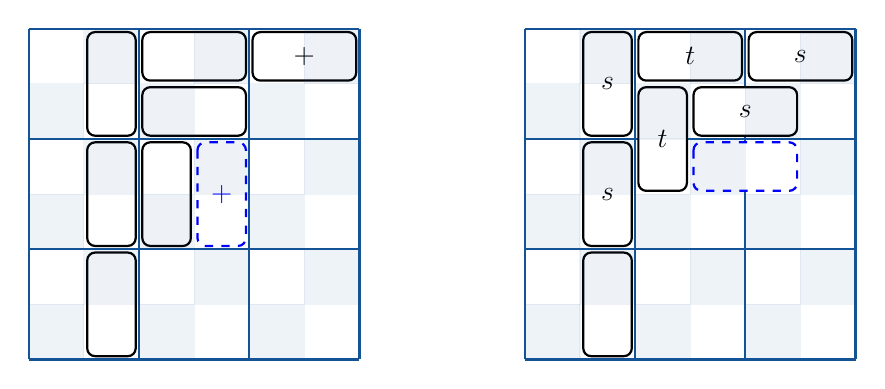
\begin{tikzpicture}[tableau, scale = .7]
            \gridLines{3}{3}
            \verticalDomino{1}{2}{ }
            \horizontalDomino{1}{3}{ }
            \horizontalDomino{1}{5}{+}
            \verticalDomino{3}{2}{ }
            \horizontalDomino{2}{3}{ }
            \verticalDomino{3}{3}{}
            \verticalDominoMaybe{3}{4}{+}
            \verticalDomino{5}{2}{ }
            \fixedSquaresForGrid{3}{3}

            \gridLinesShift{3}{3}{9}
            \verticalDominoShift{1}{2}{s}{9}
            \horizontalDominoShift{1}{3}{t}{9}
            \horizontalDominoShift{1}{5}{s}{9}
            \verticalDominoShift{3}{2}{s}{9}
            \verticalDominoShift{2}{3}{t}{9}
            \horizontalDominoShift{2}{4}{s}{9}
            \verticalDominoShift{5}{2}{ }{9}
            \horizontalDominoMaybeShift{3}{4}{ }{9}
            \fixedSquaresForGridShift{3}{3}{9}
          \end{tikzpicture}
        \end{figure}
        The effective sign of the horizontal domino directly above this square must be positive, since the added domino made it past.
        So, the sign in the domino two squares above this square must be $+$ or blank.
        If it is blank, then we need to put the $+$ sign in the top of the cycle, which we can do before  (or after) contracting.
        There won't be a shape change, since the cycle is boxed.
        \begin{figure}[H]
          \centering
          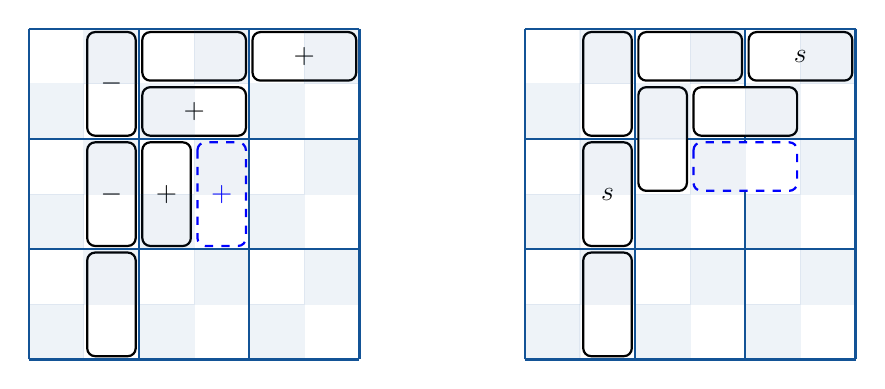
\begin{tikzpicture}[tableau, scale = .7]
            \gridLines{3}{3}
            \verticalDomino{1}{2}{-}
            \horizontalDomino{1}{3}{ }
            \horizontalDomino{1}{5}{+}
            \verticalDomino{3}{2}{-}
            \horizontalDomino{2}{3}{+}
            \verticalDomino{3}{3}{+}
            \verticalDominoMaybe{3}{4}{+}
            \verticalDomino{5}{2}{ }
            \fixedSquaresForGrid{3}{3}

            \gridLinesShift{3}{3}{9}
            \verticalDominoShift{1}{2}{ }{9}
            \horizontalDominoShift{1}{3}{ }{9}
            \horizontalDominoShift{1}{5}{s}{9}
            \verticalDominoShift{3}{2}{s}{9}
            \verticalDominoShift{2}{3}{ }{9}
            \horizontalDominoShift{2}{4}{ }{9}
            \verticalDominoShift{5}{2}{ }{9}
            \horizontalDominoMaybeShift{3}{4}{ }{9}
            \fixedSquaresForGridShift{3}{3}{9}
          \end{tikzpicture}
        \end{figure}
        Finally, we box up the new dominoes.

        \begin{figure}[H]
          \centering
          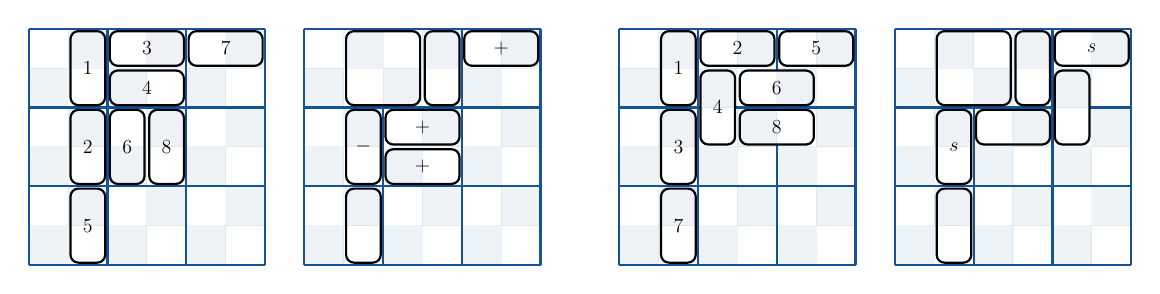
\begin{tikzpicture}[tableau, scale=.5]\gridLines{3}{3}\verticalDomino{1}{2}{1}\verticalDomino{3}{2}{2}\horizontalDomino{1}{3}{3}\horizontalDomino{2}{3}{4}\verticalDomino{5}{2}{5}\verticalDomino{3}{3}{6}\horizontalDomino{1}{5}{7}\verticalDomino{3}{4}{8}\fixedSquaresForGrid{3}{3}\gridLinesShift{3}{3}{7}\verticalDominoShift{3}{2}{-}{7}\verticalDominoShift{1}{4}{}{7}\verticalDominoShift{5}{2}{}{7}\horizontalDominoShift{4}{3}{+}{7}\horizontalDominoShift{1}{5}{+}{7}\horizontalDominoShift{3}{3}{+}{7}\emptyBoxShift{1}{2}{7}\fixedSquaresForGridShift{3}{3}{7}\gridLinesShift{3}{3}{15}\verticalDominoShift{1}{2}{1}{15}\horizontalDominoShift{1}{3}{2}{15}\verticalDominoShift{3}{2}{3}{15}\verticalDominoShift{2}{3}{4}{15}\horizontalDominoShift{1}{5}{5}{15}\horizontalDominoShift{2}{4}{6}{15}\verticalDominoShift{5}{2}{7}{15}\horizontalDominoShift{3}{4}{8}{15}\fixedSquaresForGridShift{3}{3}{15}\gridLinesShift{3}{3}{22}\verticalDominoShift{1}{4}{}{22}\verticalDominoShift{3}{2}{s}{22}\horizontalDominoShift{1}{5}{s}{22}\verticalDominoShift{2}{5}{}{22}\verticalDominoShift{5}{2}{}{22}\horizontalDominoShift{3}{3}{}{22}\emptyBoxShift{1}{2}{22}\fixedSquaresForGridShiftAlt{3}{3}{22}\end{tikzpicture}
        \end{figure}
      \end{itemize}
    \end{itemize}
  \end{itemize}


\end{document}
